\documentclass[a4paper, 11pt, titlepage]{article}

% Set page size and margins
% Replace `letterpaper' with`a4paper' for UK/EU standard size
\usepackage[a4paper,top=2.25cm,bottom=2.25cm,left=2cm,right=2cm,marginparwidth=2cm]{geometry}

% Useful packages
\usepackage{amsmath}
\usepackage{graphicx}
\usepackage[toc,page]{appendix}
\usepackage[colorlinks=true, allcolors=blue]{hyperref}
\usepackage{caption}
\usepackage{titlepic}
\usepackage{titling}
\usepackage{tikz}
\usepackage{listings}
\usepackage{xcolor}      
\usepackage{caption}
\usetikzlibrary{arrows.meta, positioning}
\usepackage{longtable}
\usepackage{wrapfig}
\usepackage{stfloats}
\usepackage{placeins}
\usepackage{subcaption} 
\usepackage{indentfirst}
\usepackage[utf8]{inputenc}
\usepackage{titlesec}
\usepackage{float}
\usepackage{tabularx}
\usepackage{subcaption}
\usepackage{pdfpages}
\titlespacing*{\section}{2em}{*1}{*1}
\titlespacing*{\subsection}{3em}{*1}{*1}
\titlespacing*{\subsubsection}{4em}{*1}{*1}

% Bibliography
\usepackage[english]{babel} 

\usepackage[%
backend=biber,
natbib=true,
urldate=iso,
seconds=ture,
style=ieee,
]{biblatex}
\addbibresource{report.bib} %Import the bibliography file

% Code style
\lstdefinestyle{cstyle}{
    language=C,
    numbers=left,
    numberstyle=\tiny\color{gray},
    numbersep=10pt,
    stepnumber=1,
    firstnumber=auto,       % Line numbers match file's
    frame=single,
    rulecolor=\color{black},
    frameround=tttt,
    backgroundcolor=\color{gray!10},
    keywordstyle=\color{blue}\bfseries,
    stringstyle=\color{red},
    commentstyle=\color{green!50!black}\itshape,
    basicstyle=\ttfamily\footnotesize,
    breaklines=true,
    captionpos=b,
    showstringspaces=false,
}

%------------------- VARIABLES -------------------%
\def\majorheading{EGH456 - Embedded Systems} % e.g. Unit name: EGH400-1 - Research Project 1
\def\minorheading{Group 17} % e.g. Group or type of report: Group 42, or Progress Report
\def\reporttitle{Embedded Systems Design for an Electric Vehicle} % e.g. My Project Title, or ROS2 on a PenguinPi
\def\reportsubtitle{Assessment 2} % (OPTIONAL - comment out to remove) e.g. Modernising Educational Robotics
\def\institutionname{Queensland University of Technology}
\def\date{30th May, 2025} % Due Date
% Authors. If there are multiple, separate by \and commands. Use \\ to separate lines within a single author's entry -- for example, to give the author's institution or address. 
\def\authorname{
    Ivan Keh - n11210656 \\
    James Prince - n10421262 \\
    Jason Tieu - n10972030 \\
    Samuel Smith - n11064196 \\
}

\title{\reporttitle}
\author{\authorname}

%-------------------------------------------------%

% Headers and footers
\usepackage{fancyhdr}
\pagestyle{fancy}
\fancyhf{}
\lhead{\reporttitle}
\rhead{\majorheading \space-\space \minorheading}
\setlength{\headheight}{13.6pt}
\addtolength{\topmargin}{-1.6pt}
\rfoot{Page \thepage}
\setlength{\parindent}{15pt}
\setlength{\parskip}{0pt}

\begin{document}

\begin{titlepage} % Suppresses displaying the page number on the title page and the subsequent page counts as page 1
\newcommand{\HRule}{\rule{\linewidth}{0.5mm}} % Defines a new command for horizontal lines, change thickness here

\center % Centre everything on the page
%------------------------------------------------
%	Logo
%------------------------------------------------

\vfill\vfill

\includegraphics[width=0.1\textwidth]{images/qut-logo.jpg}\\[1cm] % Include a department/university logo - this will require the graphicx package

%------------------------------------------------
%	Headings
%------------------------------------------------

\textsc{\LARGE \institutionname}\\[1.5cm] % Main heading such as the name of your university/college

\textsc{\Large \majorheading}\\[0.5cm] % Major heading such as course name

\textsc{\large \minorheading}\\[0.5cm] % Minor heading such as course title

%------------------------------------------------
%	Title
%------------------------------------------------

\HRule\\[0.8cm]

{\huge\bfseries \reporttitle}\\[0.4cm] % Title of your document
\ifx\reportsubtitle\undefined 
\else
    {\textsc{\Large \reportsubtitle}}\\[0.4cm] % Subtitle
\fi

\HRule\\[0.5cm]

%------------------------------------------------
%	Author(s)
%------------------------------------------------

% {\large\textit{Authors}}\\
\theauthor[0.4cm]

%------------------------------------------------
%	Date
%------------------------------------------------

\vfill\vfill\vfill % Position the date 3/4 down the remaining page

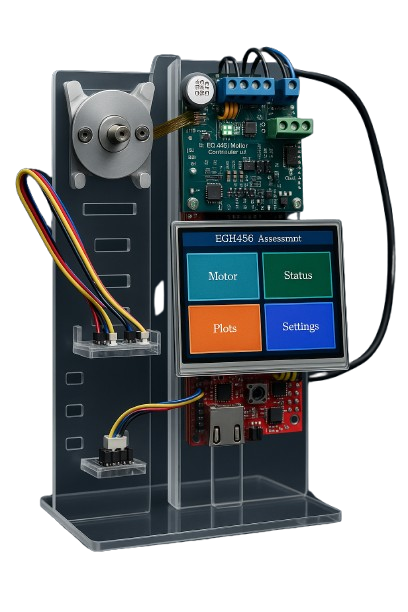
\includegraphics[width=0.43\textwidth]{images/electricVehicle-removebg.png}\\
\small\textit{Image generated by ChatGPT with a Photo of the provided Kit \parencite{openai2024}}
%----------------------------------------------------------------------------------------

	
\end{titlepage}
% \maketitle
{\hypersetup{linkcolor=black} 
% \let\clearpage\relax 
\thispagestyle{empty}
\tableofcontents
\listoffigures
\listoftables
\clearpage
}
\pagenumbering{arabic}

%------------------------------------------------
%	Reference Latex Functions
%------------------------------------------------

% ----------- Section header -----------
% \section{Importing the data}

% ----------- Section body -----------
% The first step taken in the data analysis was to import the dataset then perform preliminary checks on the data to make sure that it was imported correctly, checking that the data was of the correct type (string, numeric, date etc). As the dataset was provided in a CSV file format, the data was imported into MATLAB with the \verb_readtable_ command. Once the dataset had been imported, the first and last 100 rows of data where viewed to check the data types of the columns (Table \ref{tab:data_type}). The dataset was also observed to have 1,000,000 rows.

% ----------- Reference figures, tables, etc. with \ref (see above) -----------

% ----------- Cite bibliography source with \cite -----------
% \cite{greenwade93}

% ----------- Table -----------
% \begin{table}[h]
%     \centering
%% ----------- Table columns and sizes -----------
%     \begin{tabular}{|p{0.2\linewidth}|p{0.4\linewidth}|p{0.24\linewidth}|} 
%     \hline
%% ----------- Column names -----------
%     {Column} & {Assigned Name} & {Data type} \\ 
%     \hline
%% ----------- Column data seperated by &, line ended in \\ -----------
%     One & IV 1 & Datetime \\
%     Two & IV 2 & Numeric \\
%     Three & IV 3 & Numeric \\
%     Four & IV 4 & Numeric \\
%     Five & DV 1 or Categories & String \\
%     Six & DV 2 & Datetime \\
%     \hline
%     \end{tabular}
%     \caption{Column data types and assigned names}
%% ----------- Table label (used for references) -----------
%     \label{tab:data_type}
% \end{table}

% ----------- Figure -----------
%% For figure placement, use the following codes on \begin{figure*}[b]. b - bottom of page, t - top of page, h - here (inline), can combine in order of preference, e.g. ht prefer here then top. Can add ! to "insist" on placement, e.g. !htb.
% \begin{figure*}[b] 
% \centering
% 
\includegraphics[width=0.9\linewidth]{images/qut-logo.jpg}
% \caption{Caption}
% \label{fig:my_figure}
% \end{figure*}

% ----------- Verbatim environment used for code text ----------- 
% \begin{verbatim}
% \end{verbatim}

% ----------- Inline Maths ----------- 
% \LaTeX{} is great at typesetting mathematics. Let $X_1, X_2, \ldots, X_n$ be a sequence of independent and identically distributed random variables with $\text{E}[X_i] = \mu$ and $\text{Var}[X_i] = \sigma^2 < \infty$, and let
% $$S_n = \frac{X_1 + X_2 + \cdots + X_n}{n}
%       = \frac{1}{n}\sum_{i}^{n} X_i$$
% denote their mean. Then as $n$ approaches infinity, the random variables $\sqrt{n}(S_n - \mu)$ converge in distribution to a normal $\mathcal{N}(0, \sigma^2)$.

% ----------- Multiline equations (aligned) ----------- 
%% Align single equation
% \begin{equation} \label{eq1}
% \begin{split}
% A & = \frac{\pi r^2}{2} \\
%  & = \frac{1}{2} \pi r^2
% \end{split}
% \end{equation}

%% Aligning several equations
% \begin{align*} 
% 2x - 5y &=  8 \\ 
% 3x + 9y &=  -12
% \end{align*}

%% Aligning several equations (multiple columns)
% \begin{align*}
% x&=y           &  w &=z              &  a&=b+c\\
% 2x&=-y         &  3w&=\frac{1}{2}z   &  a&=b\\
% -4 + 5x&=2+y   &  w+2&=-1+w          &  ab&=cb
% \end{align*}

%% Grouping and centering equations
% \begin{gather*} 
% 2x - 5y =  8 \\ 
% 3x^2 + 9y =  3a + c
% \end{gather*}

% ----------- Lists ----------- 
% You can make lists with automatic numbering \dots. Start typing \enumerate or \itemize, then tab to autocomplete for a shortcut.
% \begin{enumerate}
% \item Like this,
% \item and like this.
% \end{enumerate}
% \dots or bullet points \dots
% \begin{itemize}
% \item Like this,`1
% \item and like this.
% \end{itemize}

%------------------------------------------------
%	Main Report
%------------------------------------------------

\section{Introduction}
Electric vehicles (EVs) are becoming increasingly common as the world seeks cleaner and more efficient alternatives to traditional combustion engines. This shift introduces significant engineering challenges in the design of embedded systems that can safely and efficiently control electric motors under real-time constraints. Unlike internal combustion engines, electric motors require fine-grained, rapid control of torque and speed, and the systems supporting them must be capable of immediately responding to changes in load, velocity, and external conditions.\\

This project focuses on the development of a real-time embedded system for controlling a three-phase Brushless DC (BLDC) motor and providing live feedback to the user via a touchscreen graphical interface. In automotive applications, such systems must operate under strict timing constraints, where delayed responses to critical events, such as obstacle detection or electrical faults, can lead to unsafe behaviour or physical damage. Ensuring safe and reliable vehicle operation therefore requires deterministic system behaviour, where tasks are executed predictably and safety mechanisms respond within guaranteed time bounds. This places significant demands on embedded software design, particularly in coordinating concurrent processes such as motor control, sensor acquisition, and fault handling under real-time constraints.  \\

The embedded platform selected for this project is the Tiva TM4C1294NCPDT microcontroller, which supports high-performance real-time applications with its ARM Cortex-M4F core and extensive peripheral interfaces. The system architecture is built around FreeRTOS, enabling pre-emptive multitasking for concurrent execution of motor control, sensor acquisition, safety monitoring, and user interface tasks. A modular software structure is employed to ensure maintainability, while UART telemetry and SerialPlot are used to visualise system performance for debugging and validation.\\

The embedded software must meet several key requirements:
\begin{itemize}
    \item Real-Time Performance\textbf{:} Ensures timely execution of motor control and safety routines under concurrent task loads.
    \item Motor Control and Monitoring\textbf{:} Provides smooth start-up, regulated speed control, and braking using PWM, with real-time feedback on motor RPM and power consumption.
    \item Safety and Fault Handling\textbf{:} Detects over-current, initiating emergency stop procedures and system protection.
    \item Sensor Integration\textbf{:} Acquires and filters signals from current, speed, and one optional environmental sensor, ensuring reliable data even in the presence of noise.
    \item User Interface Integration\textbf{:} Delivers a responsive graphical interface for motor control, parameter configuration, and system status visualisation, including real-time plotting of filtered data.

\end{itemize}
The final embedded system integrates these features into a cohesive and safety-aware control platform suitable for modern electric vehicle applications. The successful development of this system required coordinated efforts across multiple areas, including motor control, sensor integration, fault handling, user interface design, and system-level integration. Each team member was responsible for specific subsystems and contributed to the overall functionality, robustness, and performance of the final solution. \\

James Prince developed the motor control subsystem, including PWM regulation, RPM feedback, and UART telemetry. Samuel Smith handled sensor acquisition and filtering for speed and current data. Ivan Keh implemented fault detection and emergency stop logic. Jason Tieu designed the graphical user interface, integrating controls, status indicators, and live data plots. System integration and testing were carried out collaboratively. 
 
\section{Design and Implementation}
The system was developed using a task-based architecture built on FreeRTOS, allowing the motor control, sensor processing, and user interface components to operate concurrently. Each subsystem was implemented as an independent thread with clearly defined responsibilities, scheduled according to   priority and timing requirements. Inter-task communication was managed using FreeRTOS message queues for data sharing and semaphores for mutual exclusion when accessing shared resources. This structure ensured consistent and predictable system behaviour during runtime, particularly under load. \\

To support development and maintainability, comprehensive code documentation was generated using Doxygen. This automated documentation system provides detailed descriptions of all functions, and data structures, creating extensive reference materials for the codebase. The complete documentation is accessible online at \url{https://james712346.github.io/EGH456Project/}, facilitating code review, debugging, and future development efforts.\\

\begin{figure}[h!]
    \center
    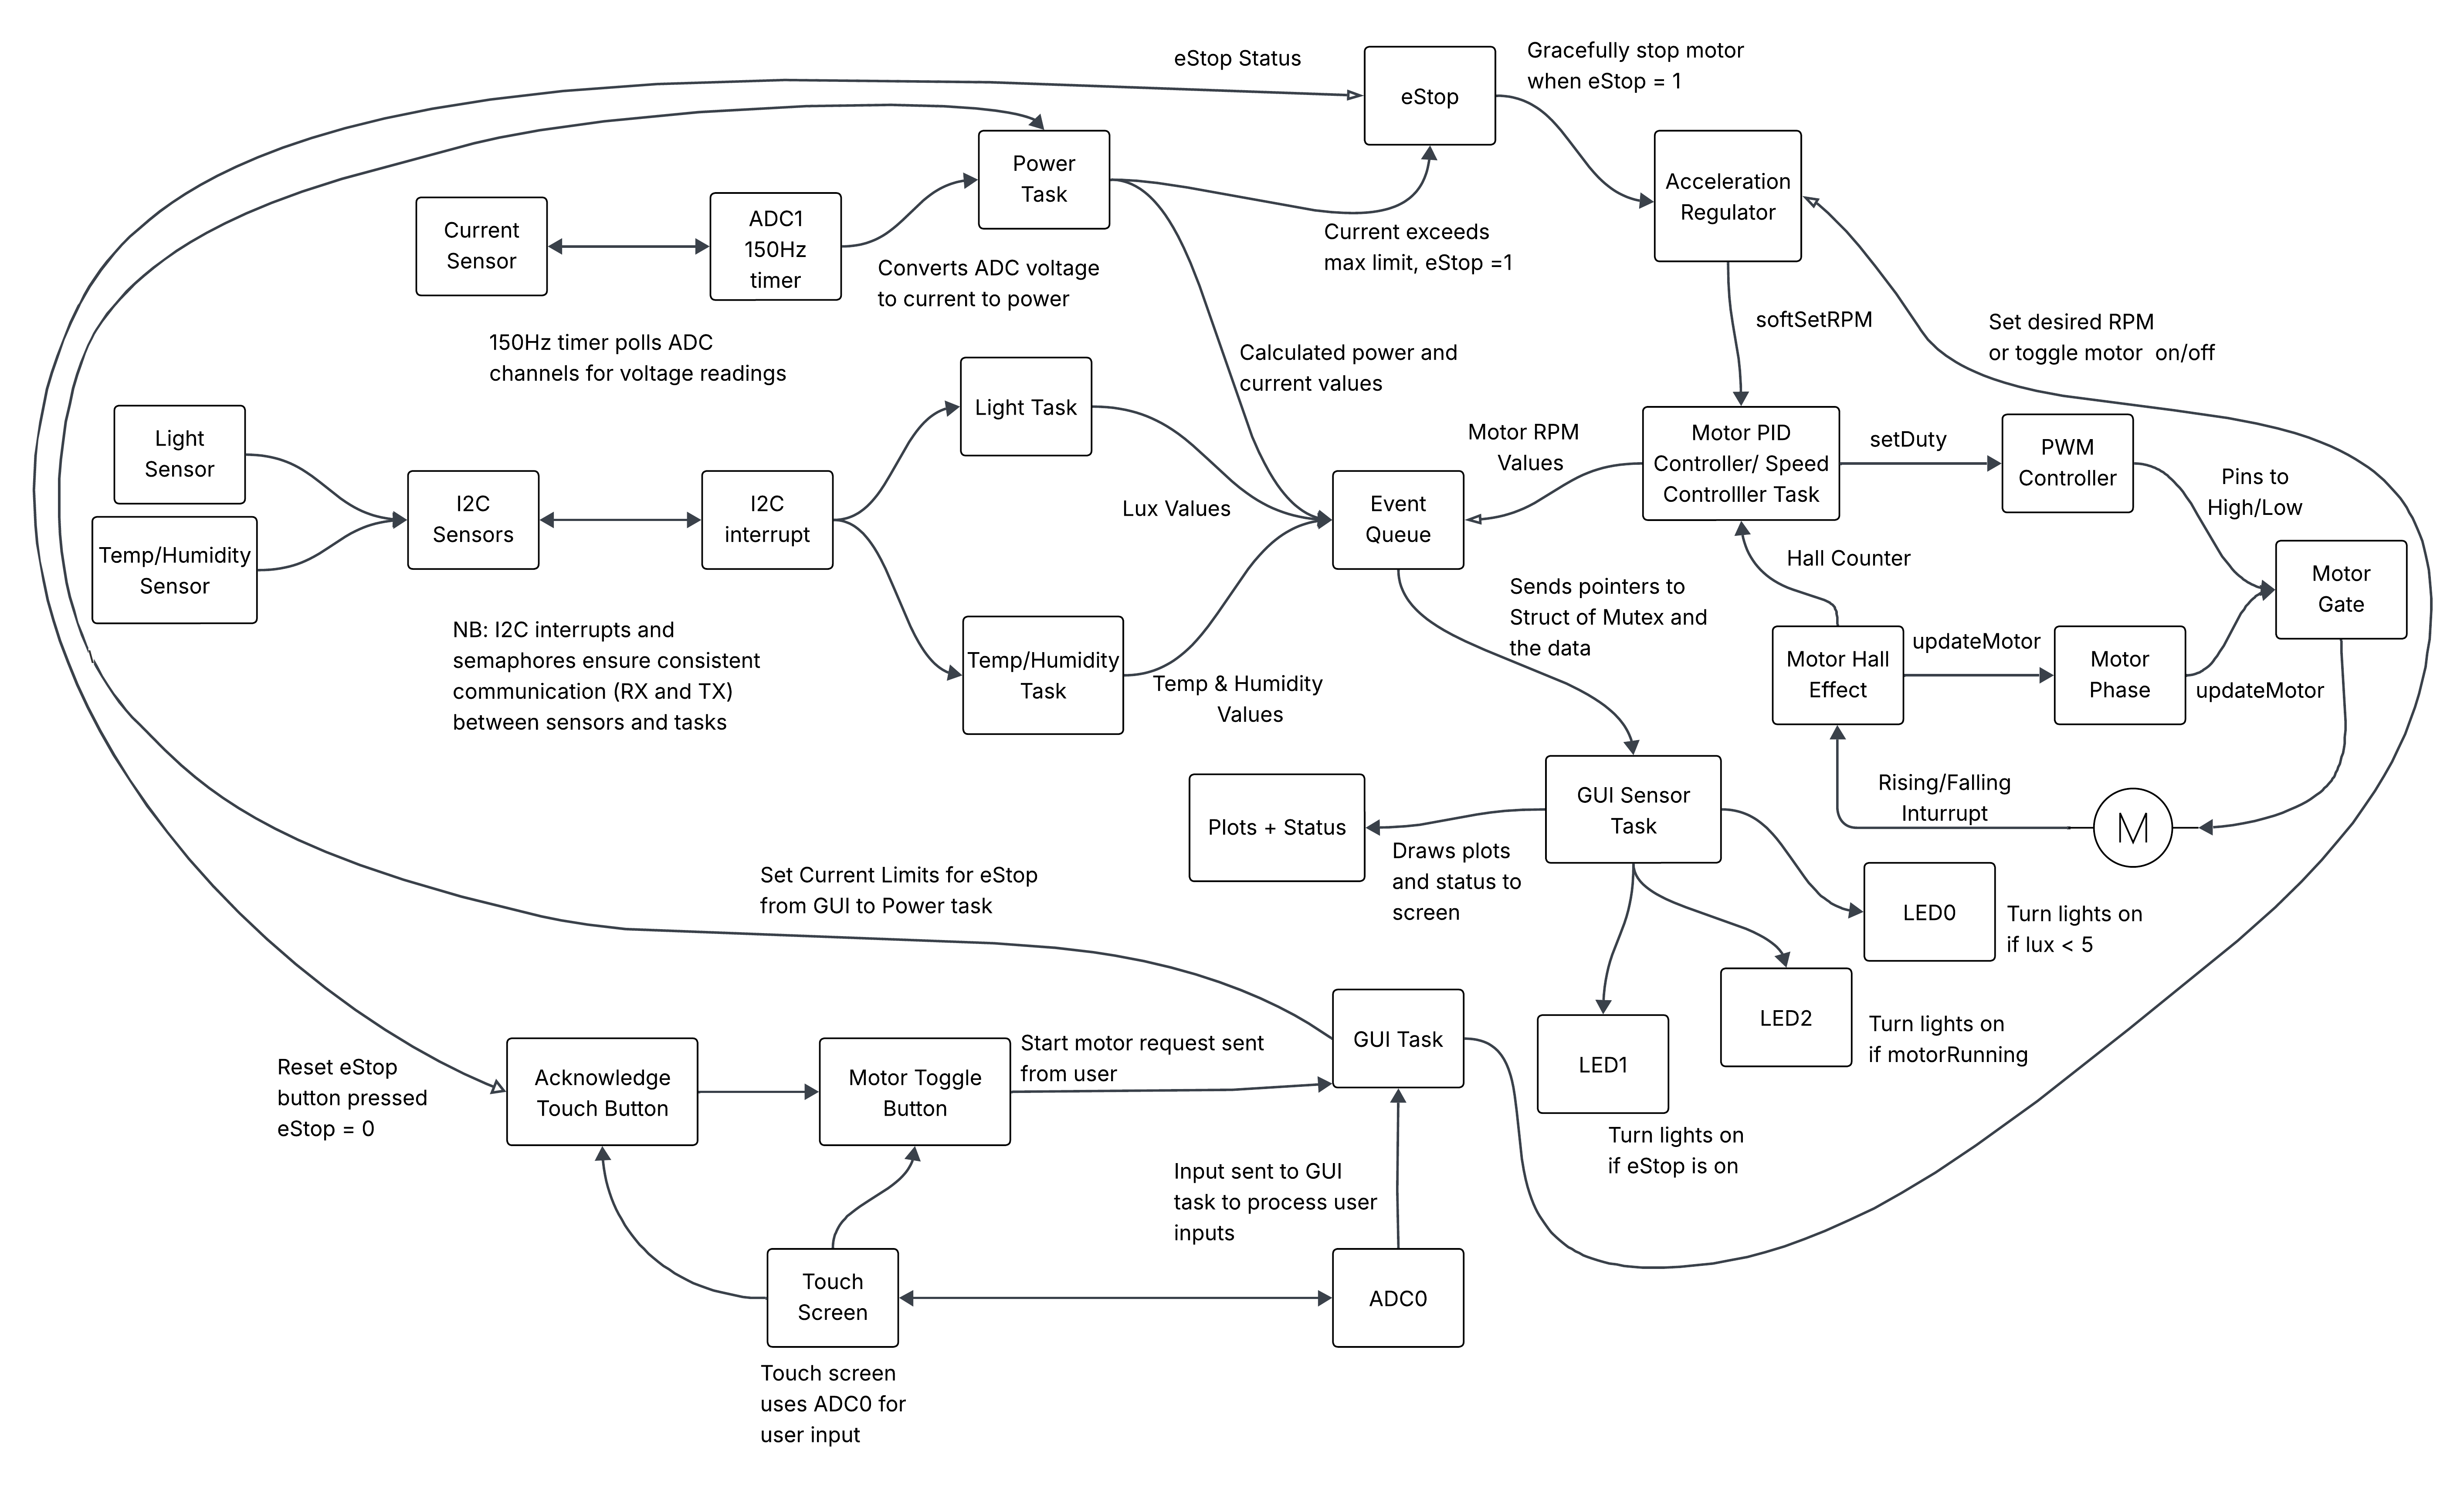
\includegraphics[width=0.7\linewidth]{images/systemArch.png}
    \caption{System architecture (Found in Appendix \ref{appendix:sysarch})}
    \label{fig:sysarch}
\end{figure}

Figure \ref{fig:sysarch} presents an overview of the RTOS task structure and system architecture, highlighting the relationships between tasks and the flow of control and data throughout the system. The following sections detail the implementation and design considerations of each major subsystem, including the motor control logic, digital signal processing for sensors, and graphical user interface integration.\\



\subsection{Shared Resources}
Our team implemented a thread-safe data sharing mechanism to enable communication between FreeRTOS tasks without blocking operations. This solution uses a two-tiered structure design combined with mutex protection to ensure data integrity in a concurrent environment.

\subsubsection{Data Structure Design}
The implementation employs two complementary structures as shown in Figure \ref{fig:shared_structs}:

\begin{enumerate}
    \item \textbf{struct val} - A simple data container with two fields: \verb|filtered| for processed sensor data and \verb|raw| for unprocessed sensor readings.
    \item \textbf{struct sharedValues} - A wrapper structure that encapsulates a \verb|val| struct containing the actual data and a mutex handle for thread-safe access control.
\end{enumerate}

This hierarchical approach separates data storage from synchronisation concerns, promoting clean code organisation and maintainability.

\begin{figure}[h!]
\centering
\begin{minipage}{0.5\linewidth}
\lstinputlisting[style=cstyle, firstline=9,firstnumber=9, lastline=17]{../include/shared.h}
\end{minipage}
\caption{Shared data structures from "/include/shared.h"}
\label{fig:shared_structs}
\end{figure}

\subsubsection{Inter-Task Communication}
For GUI updates, the system uses a FreeRTOS queue that passes pointers to initialised shared variables. This design allows the GUI task to identify specific shared resources by comparing pointers and execute the appropriate access functions without copying large data structures, improving both performance and memory efficiency.

\subsubsection{Access Functions}
The shared resource system provides three main access functions, each designed for specific use cases. Figure \ref{fig:getter_example} demonstrates the implementation of the getter function:

\begin{figure}[h!]
\centering
\begin{minipage}{0.8\linewidth}
\lstinputlisting[style=cstyle, firstline=35,firstnumber=35, lastline=42]{../src/shared.c}
\end{minipage}
\caption{Example getter function implementation from "/src/shared.c"}
\label{fig:getter_example}
\end{figure}

\paragraph{Getter Function}
Retrieves data from shared resources safely. It accepts a pointer to the target \verb|sharedValues| struct, a maximum delay for mutex acquisition, and a pointer to the buffer where retrieved data will be stored. The function safely copies current data values to the provided buffer.

\paragraph{Setter Function}
Replaces entire data content in shared resources atomically. It takes a pointer to the target \verb|sharedValues| struct, a maximum delay for mutex acquisition, and a \verb|val| struct containing new data to replace existing values. This function updates both filtered and raw values simultaneously.

\paragraph{SetterVal Function}
Updates individual data fields selectively for fine-grained control. It accepts a pointer to the target \verb|sharedValues| struct, a maximum delay for mutex acquisition, a double value to be assigned, and a boolean flag (1 = update filtered value, 0 = update raw value). This function modifies only the specified field while preserving the other.

\subsubsection{Thread Safety and Performance}
All access functions implement mutex-based synchronisation with configurable timeout periods. This approach ensures data integrity by preventing race conditions during concurrent access, while timeout mechanisms prevent indefinite blocking and potential deadlocks. The implementation ensures that tasks do not hold onto mutexes for extended periods by requiring tasks to provide pre-allocated buffers for data retrieval or pre-computed values for data updates. This design minimises the critical section duration, as tasks perform expensive computations outside the mutex-protected region and only briefly acquire the lock for fast memory copy operations. The maximum delay parameter allows each task to specify its tolerance for waiting, enabling priority-based resource access and preventing high-priority tasks from being indefinitely blocked by resource contention. This efficient design maintains system responsiveness while supporting multiple tasks safely accessing shared resources, crucial for the real-time performance requirements of the electric vehicle control system. \parencite{freertos}

\subsection{Motor}
The motor control subsystem represents one of the most critical components in the overall system architecture, as it serves as the primary output actuator capable of directly impacting user safety in a fully implemented electric vehicle. The potential for serious harm or fatality necessitates that all motor operations be designed with comprehensive safety protocols and fail-safe mechanisms as the primary consideration.\\
This section covers the complete motor control implementation, including phase switching, RPM calculations, speed control, and safety requirements.
\subsubsection{Design and Task Approach}
The Motor Subsystem was designed using two FreeRTOS tasks: one for motor control and another for RPM calculation. It incorporated three GPIO interrupt handlers, each responsible for monitoring a specific input and updating one of three bits in a $uint8\_t$ status variable based on the input’s state. The motor control task utilised Timer 1A \parencite{tm4c129ncpdt} on the micro controller to incrementally adjust the motor speed toward the user-defined target RPM, ensuring a safe and controlled acceleration. Additionally, emergency stop detection and handling were implemented within the Timer 1A interrupt, allowing immediate response to stop conditions without needing to wait for a mutex to be taken/given.
\subsubsection{Phase Timings}
The phase timings are determined using Hall effect sensors embedded in the motor, which detect the rotor's position relative to the three stator phases. Interrupts are configured on both the rising and falling edges of the H2, M3, and N2 pins \parencite{egh456support}. When triggered, these interrupts release a semaphore that activates the motor control FreeRTOS task. This task is responsible for switching the motor phases based on the currently active Hall effect sensor state.

The Hall sensors correspond to the motor phases as follows: H2 corresponds to Phase B, N2 to Phase C, and M3 to Phase A. Phase updates are handled through the provided motor API code \parencite{egh456support, drv8323}. Special consideration is given to edge cases where two Hall effect sensors are active simultaneously; these conditions are detected and correctly resolved within the custom motor control logic.

Figure~\ref{fig:hall_sensors} shows the output of the Hall effect sensors during manual rotation of the motor, demonstrating the sequence of sensor activations and their role in determining rotor position.

\begin{figure}[h]
    \centering
    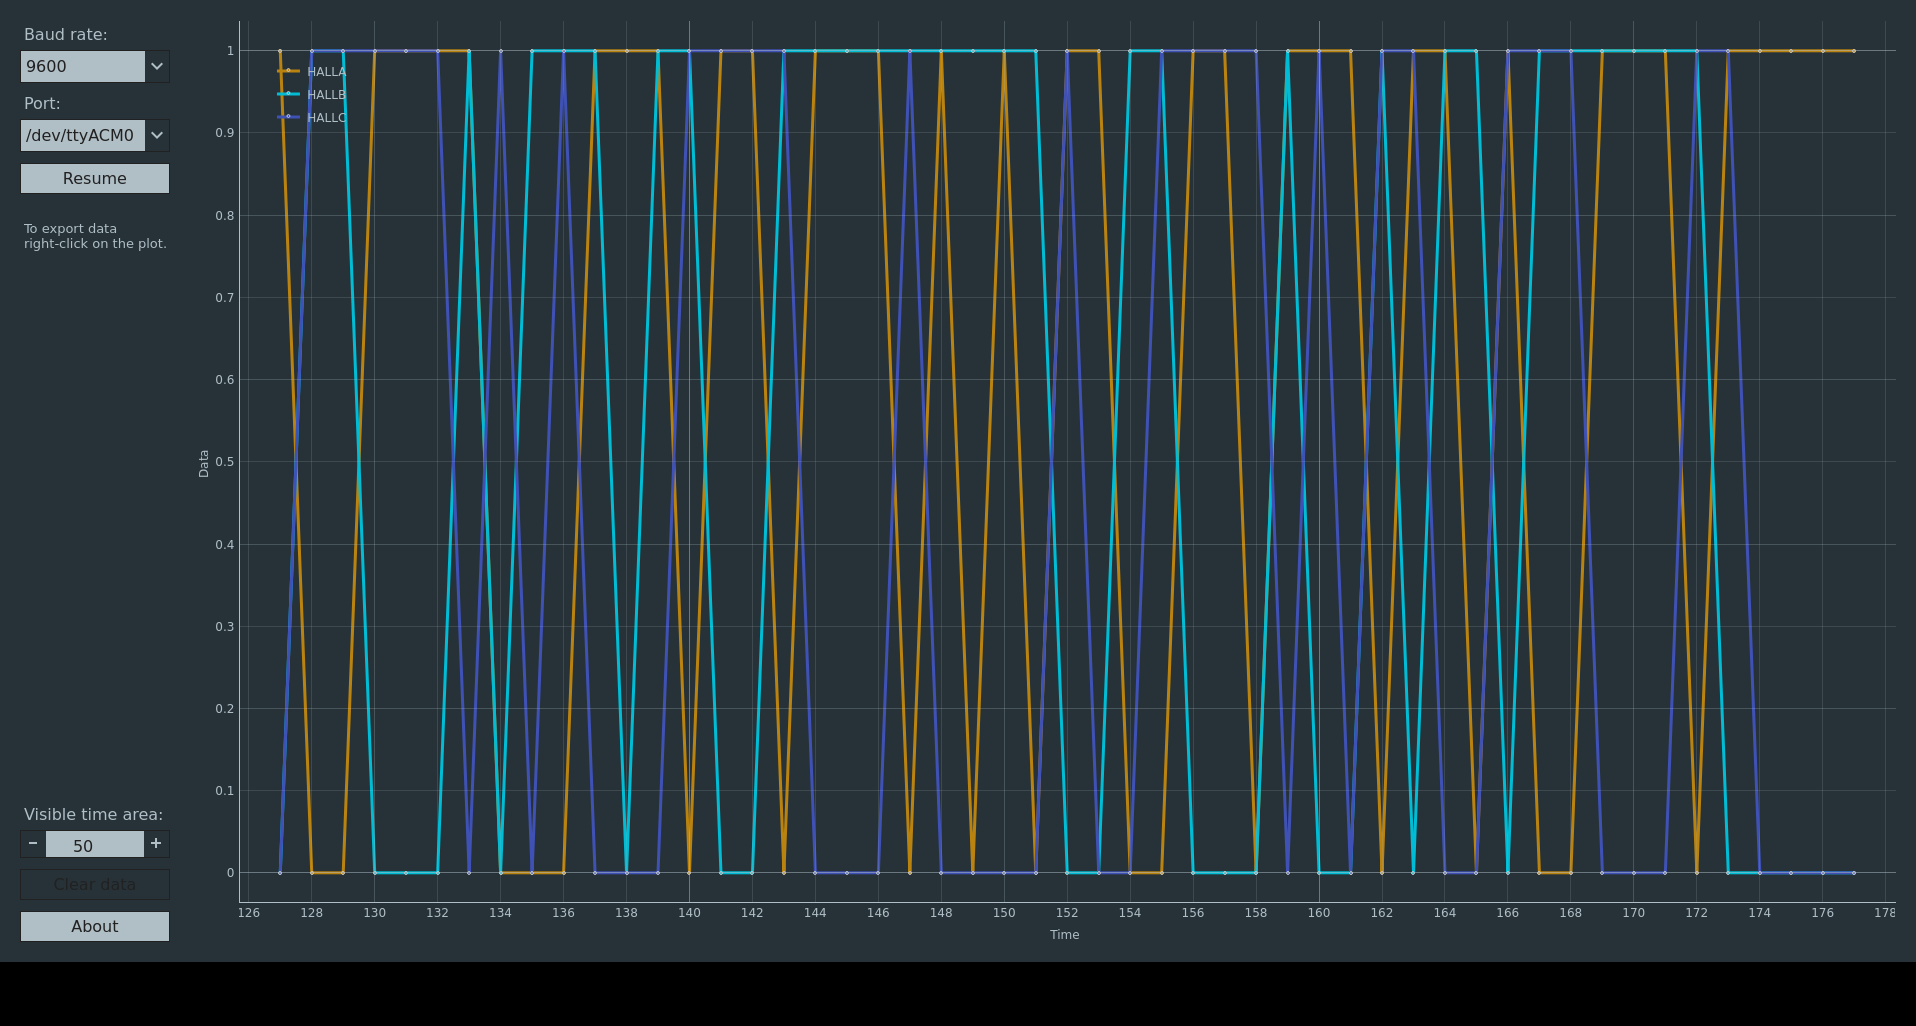
\includegraphics[width=0.6\textwidth]{images/hallEffectMadness.png}
    \caption{Hall effect sensor outputs (H2 - HALLB, M3 - HALLA, N2 - HALLC) during manual rotation of the motor.}
    \label{fig:hall_sensors}
\end{figure}

\subsubsection{Speed Calculation}
Speed calculation is performed within the speed controller task, which runs at a fixed interval. Each time the task executes, it calculates the motor speed based on the number of Hall effect rising edges that occurred since the last execution. These edges are counted by an interrupt service routine, which increments a counter on each rising edge.

The time difference \textit{dt} is calculated using \texttt{xTaskGetTickCount()}, which returns the number of ticks since the system started. The speed controller task stores the tick count from its previous execution and subtracts it from the current tick count to determine \textit{dt}, the elapsed time in milliseconds.

Given that there are 12 Hall effect triggers per revolution\parencite{motordata}, the rotational speed in RPM is calculated using the following equation:

\begin{equation}
    \text{RPM} = 60 \times \frac{a}{12} \times \frac{1000}{dt}
\end{equation}

Where:
\begin{itemize}
    \item $a$ is the number of Hall effect rising edges counted since the last task execution,
    \item $dt$ is the time difference between the current and previous executions of the speed controller task, in milliseconds.
\end{itemize}
\subsubsection{PID Controlller}
The PID (Proportional–Integral–Derivative) controller is a widely used feedback control mechanism designed to ensure that a system's output follows a desired reference or set point. It achieves this by continuously calculating an error value as the difference between the desired set point and the actual process variable, and applying corrective actions based on three gains \parencite{pidController}:
\begin{itemize}
    \item \textbf{Proportional ($K_p$):} Produces an output that is directly proportional to the current error. This helps drive the system toward the set point and provides an immediate correction.
    \item \textbf{Integral ($K_i$):} Accounts for the accumulation of past errors over time. It helps eliminate steady-state error by integrating the error, ensuring the output eventually reaches the set point.
    \item \textbf{Derivative ($K_d$):} Predicts the future trend of the error by considering its rate of change. It helps dampen the response and reduce overshoot.
\end{itemize}

Through motor tuning, suitable values for the proportional and integral gains were selected, while a small derivative gain was also introduced to improve stability.

The PID controller was implemented within the speed controller task and executed after each speed calculation. This placement allows the system to respond quickly to any sudden changes in load or target speed. To avoid instability during startup or low-speed operation, the PID calculation was conditionally skipped when the motor was off or operating below 100 RPM. In these cases, a kick-start mechanism was used to help the motor begin spinning before engaging the PID controller, preventing erratic control behaviour.
\subsubsection{Safety Acceleration Considerations}
Acceleration is managed using Timer 1A on the micro controller, which is configured to run at 50~Hz. On system startup, a step size is calculated by dividing the maximum allowed RPM acceleration by the timer frequency. For this project, the requirement is a maximum acceleration of 500~RPM/s, resulting in step increments of $\pm 10$~RPM per timer interrupt.

These step changes are applied to a variable referred to as the \textit{soft RPM}, which incrementally approaches the user-defined target RPM. The soft RPM is then passed to the PID controller. This approach ensures smooth and controlled acceleration and deceleration, preventing sudden changes in speed that could hurt a passenger.

Figure~\ref{fig:rpm_acceleration} illustrates the behaviour of the acceleration logic. The plot shows the measured RPM and the soft RPM over time. The staircase-like pattern of the soft RPM highlights the discrete step increments applied at each timer interrupt. The measured RPM follows this curve as the PID controller adjusts the motor output accordingly.

\begin{figure}[h!]
    \centering
    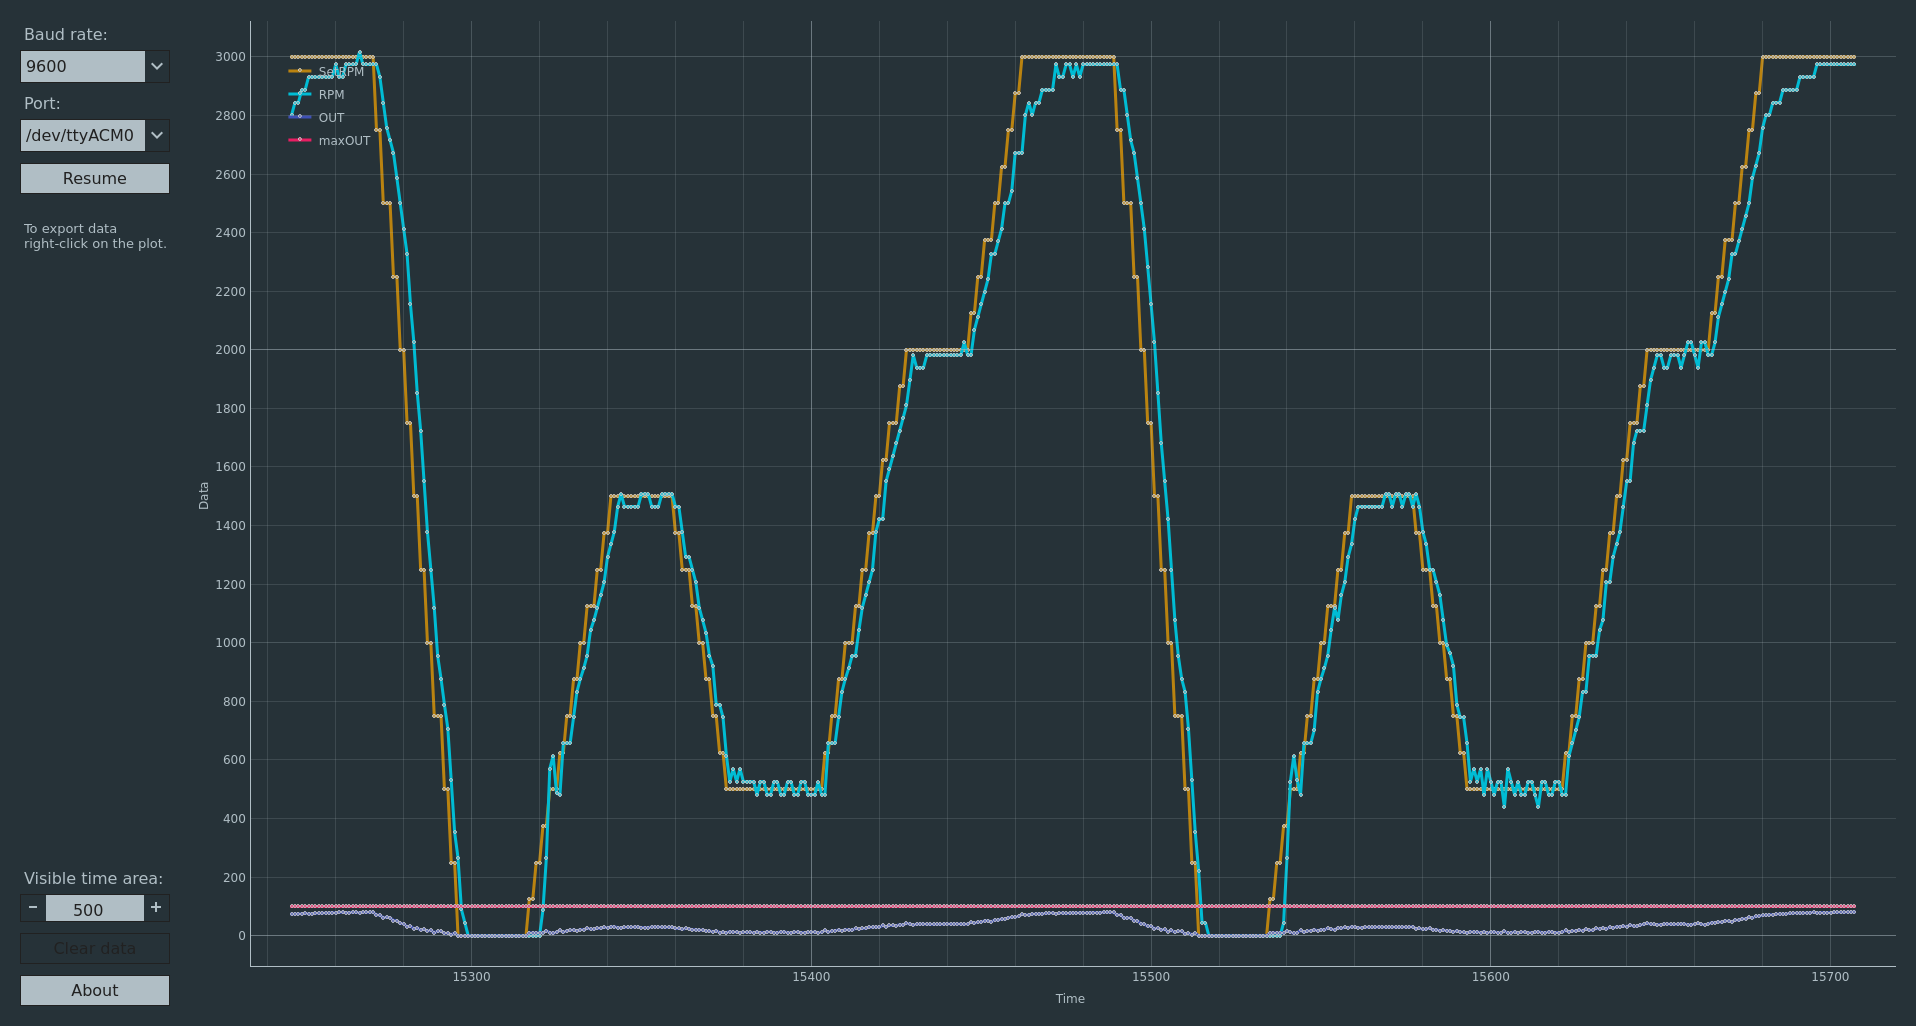
\includegraphics[width=0.85\textwidth]{images/accel.png}
    \caption{Measured RPM vs. Soft RPM over time}
    \label{fig:rpm_acceleration}
\end{figure}
\subsubsection{Emergency Stop}
The Emergency Stop (e-stop) is a system requirement that demands the motor decelerate to a complete stop at a rate of 1000~RPM/s. Leveraging the same logic used for normal acceleration, the system switches to a more aggressive step size when an e-stop condition is detected. Specifically, within the Timer 1A interrupt, the step value is adjusted to match the required e-stop deceleration, and the target RPM is immediately set to 0.

Because this logic is handled inside the timer interrupt, it avoids the need for mutexes or coordination with other tasks. The code is kept minimal to prevent blocking the rest of the system. As shown in Figure~\ref{fig:rpm_acceleration} around the 15,500~time mark, the system exhibits a rapid decrease in RPM, with larger downward steps to zero that is clearly contrasting the gradual transitions seen during normal operation.
\subsubsection{Interfacing with Additional Tasks}
To interface with other tasks in the system, we publish current RPM, set RPM, and output using the shared value structures described earlier. These values are pushed to a FreeRTOS queue whenever they are updated. 

For the emergency stop (e-stop), we implemented a dedicated setter and getter function that is shared between the GUI and sensor tasks. This allows tasks to easily and safely trigger or detect whether an e-stop condition has occurred.


\newpage
\subsection{Sensors}
Multiple sensors have been implemented in the design to monitor various conditions both inside and outside the system. Temperature and humidity sensors measure the temperature in degrees Celsius and the humidity in Relative Humidity, while a light sensor measures the ambient light levels in lux. The system measures the voltage of two of the three voltage sensors, converts it to a current reading, and calculates the power drawn from the motor. Speed sensing was done using the Hall Effect sensors connected to GPIO pins. This section will summarise the integration of sensors into the system.

\subsubsection{Design and Task Approach}
The sensor subsystem was designed to collect sensor data using two main sources, ADC and I2C. Light \parencite{opt3001}, temperature, and humidity were collected from the sensors that interface with I2C, while the speed and current sensors used ADC to gather data necessary for their sensor outputs. The hardware connections for I2C needed to be confirmed to ensure that the correct lines were setup for I2C sensor communication \parencite{boosterpack}. Once that had been established, testing of the initial communications to each sensor was the nest step towards this task. The light and climate sensors required initialisation before sensor data could be collected. By ensuring that initialisation completed correctly, could the data gathered from the sensors be analysed. Testing of light values was done by flashing a light at the sensor and watching the values change over UART, while temperature and humidity was similarly tested by warming the sensor and breathing on it to see sensor values change over UART.\\

For the ADC collection, the hardware connections had to be established to ensure that the proper pins were configured for ADC. While hardware connection diagrams were provided showing what pins were connected to the voltage lines, an ADC scan task function was created to poll all of the ADC lines to ensure readings were suitable from a voltage sensor. The datasheet explains that the voltage is bidirectional, so a zero voltage reading would be halfway between the 4095 max ADC voltage reading. Once those lines had been identified using the ADC scan task and the hardware connection diagrams, the formula provided in the motor data sheet \parencite{drv8323} was used to convert the voltage readings to current. By multiplying the 24V motor voltage by the current, and multiplying those results by 1.3 (to account for only having 2/3 of the voltage reading), a power measurement was possible. \\

% (Talk about speed sensing here? James?) k
The speed sensing was achieved by using the three hall effect sensors connected to GPIO pins M, H, and N. These sensors generated interrupts on both the rising and falling edges, with each full revolution of the motor producing 12 transitions. An interrupt service routine (ISR) incremented a transition counter, which was sampled by the speed controller task to calculate RPM. The PID controller was able to use this feedback for precise motor feedback. \\

\subsubsection{Sensor Hardware Overview}

The sensor subsystem incorporates multiple devices to monitor environmental conditions, motor behaviour and safety parameters. Table~\ref{tab:sensor-overview} provides a summary of the sensors implemented into the system, their types, interfaces and respective purposes with the system.

\begin{table}[H]
    \centering
    \caption{Sensor Hardware Overview}
    \label{tab:sensor-overview}
    \begin{tabularx}{\textwidth}{|l|l|l|X|}
    \hline
    \textbf{Sensor} & \textbf{Type} & \textbf{Protocol} & \textbf{Purpose} \\ \hline
    OPT3001 & Ambient Light Sensor & I2C & Detect lighting conditions for day/night \\ \hline
    SHT31 & Temperature \& Humidity & I2C & Environmental monitoring \\ \hline
    ADC Channels 0 \& 4 & Current Sensing (2 Phases) & ADC Interrupts & Monitor motor current using 7m$\Omega$ shunts (dual phase, 1.3x correction factor) \\ \hline
    Hall Effect Sensors A, B, C & Speed Sensing & GPIO Interrupts & Measure motor RPM using Hall edge counting (12 transitions per revolution) \\ \hline
    \end{tabularx}
\end{table}
The sensors that have been selected allow comprehensive monitoring of the environment and motor parameters while balancing system complexity and real-time constraints within the system. The following sections will cover the details surrounding the integration of sensors into the system.\\
\subsubsection{Connection Overview}
The OPT3001 ambient light sensor and the SHT31 temperature and humidity sensor \parencite{sht31} shared the I2C bus, each with their own unique device addresses. The micro controller polls each sensor via their own dedicated FreeRTOS sensor task. The ADC-based current sensing and hall effect speed sensing operate independently of the I2C bus. MCU interface connections can be seen in Table~\ref{tab:connection-overview}\\

\begin{table}[H]
    \centering
    \caption{Connection Overview}
    \label{tab:connection-overview}
    \begin{tabularx}{\textwidth}{|l|l|l|X|}
    \hline
    \textbf{Sensor} & \textbf{Protocol} & \textbf{MCU Interface} & \textbf{Notes} \\ \hline
    OPT3001 & I2C & I2C0 & Ambient Light \\ \hline
    SHT31 & I2C & I2C0 & Temperature and Humidity \\ \hline
    ADC Channels 0 \& 4 & ADC & ADC1 Ch0, Ch4 & Current monitoring \\ \hline
    Hall Effect Sensors A, B, C & GPIO & GPIO Ports M, H, N & Speed sensing \\ \hline
    \end{tabularx}
\end{table}

To identify the connections required to communicate with the sensors over I2C the booster pack pinout diagram was analysed as seen in Figure~\ref{fig:i2c-connections} showing the pins connected to the data and clock lines \parencite{boosterpack} \parencite{ek-tm4c1294xl} \parencite{tm4c129ncpdt}.\\

\begin{figure}[H]
    \centering
    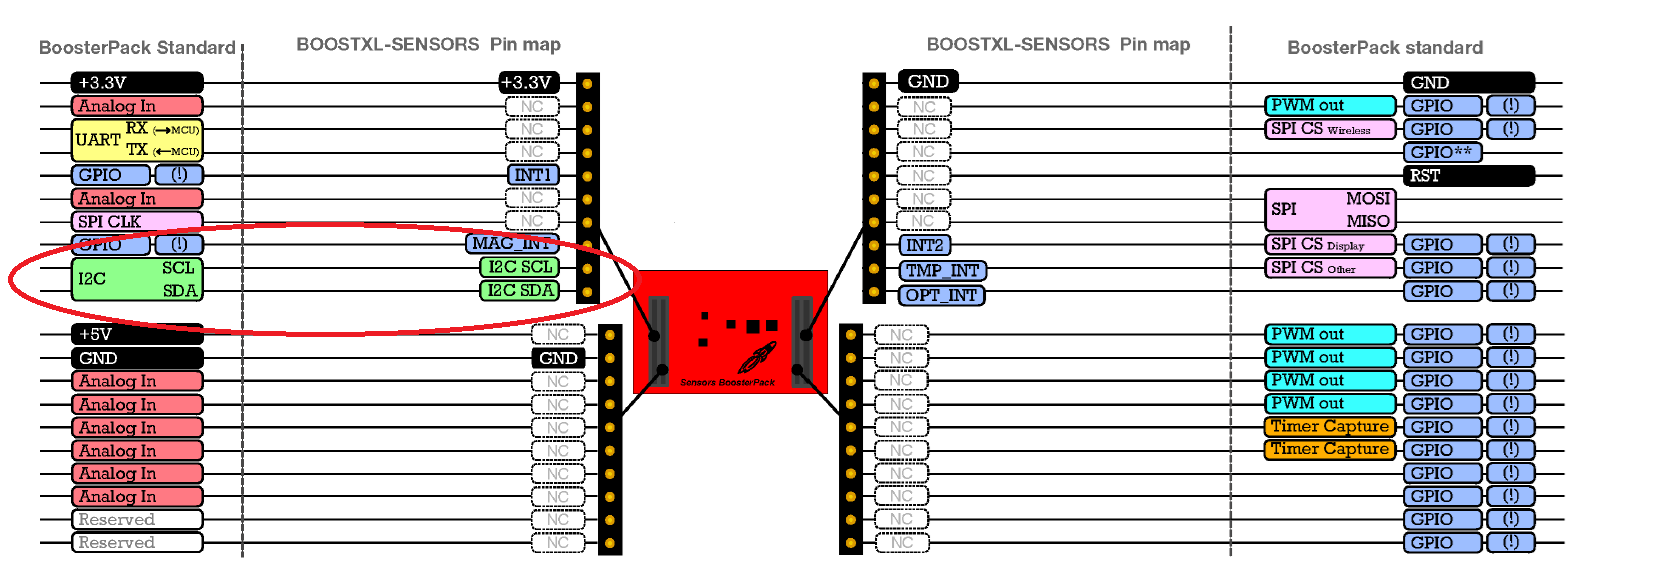
\includegraphics[width=0.8\linewidth]{images/I2C_connections.png}
    \caption{I2C Bus Connection Diagram showing I2C data and clock lines circled in red from BOOSTXL-SENSORS Sensors BoosterPack Plug-in
    Module datasheet}
    \label{fig:i2c-connections}
\end{figure}

To properly configure the hall effect sensors and the voltage lines for the motor, the pin-out diagram for the booster pack was analysed, as seen in Figure~\ref{fig:motor-connections}, showing voltage sensors on channels 0 and 4 and Hall effect sensors tied to GPIO ports M, H and N \parencite{egh456support}.\\

\begin{figure}[H]
    \centering
    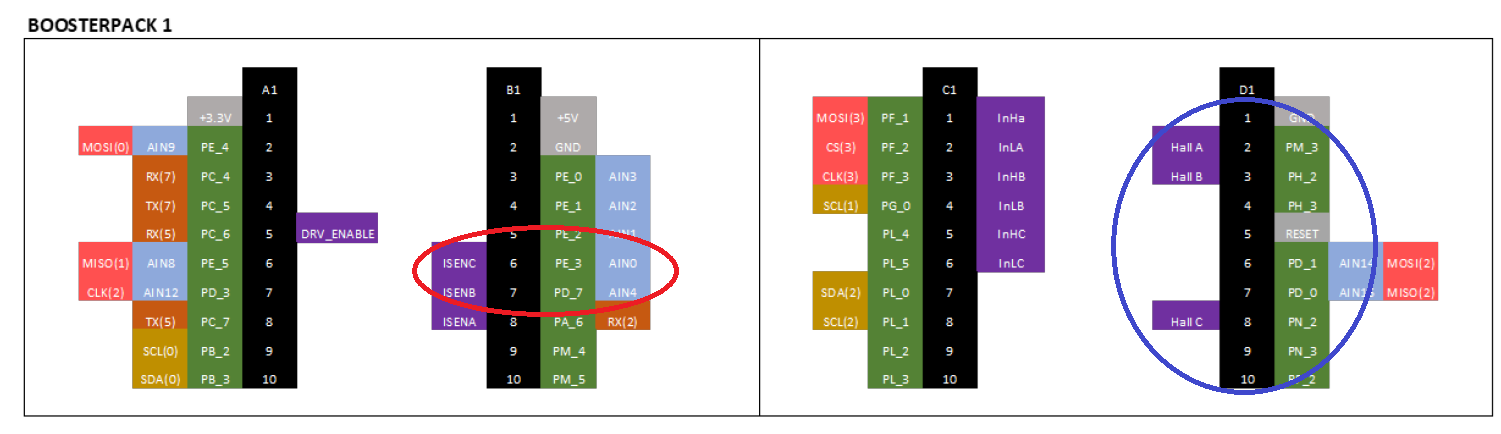
\includegraphics[width=0.8\linewidth]{images/Motor_connections.png}
    \caption{Booster Pack 1 diagram showing motor voltage lines and ports circled in red and Hall effect sensor and ports circled in blue. Sourced from unit support material.}
    \label{fig:motor-connections}
\end{figure}

% System level diagram showing sensors?

\subsubsection{FreeRTOS Sensor Task Design}

Each sensor was split up into their own subsequent FreeRTOS tasks \parencite{freertos} to ensure separation of functionality and allow setting of individual sensor timing requirements. Task call frequencies and their scheduling can be seen in Table \ref{tab:rtos-tasks}.

\begin{table}[H]
    \centering
    \caption{FreeRTOS Task Overview}
    \label{tab:rtos-tasks}
    \begin{tabularx}{\textwidth}{|l|l|X|l|}
    \hline
    \textbf{Task} & \textbf{Function} & \textbf{Polling Interval} & \textbf{Priority} \\ \hline
    Light Sensor Task & Polls OPT3001 via I2C & 500 ms & 2 \\ \hline
    Temp/Humidity Task & Polls SHT31 via I2C & 1000 ms & 3 \\ \hline
    Power Task & Reads ADC Ch0/Ch4, computes current & 100 ms & 8 \\ \hline
    Speed Controller Task & Calculates RPM and PID control & 100 ms & 9 \\ \hline
    \end{tabularx}
\end{table}

Each task was assigned their RTOS priority based on their call frequency, sensor polling requirements and their importance to system functionality. Light and climate sensors were given lower task priorities compared to the Power and Speed controller tasks due to their critical functions of handling motor functionality and monitoring current limits.\\

To ensure that I2C read and write communication was consistent, a semaphore was used to ensure that timing requirements were met throughout I2C transmissions.


\subsubsection{Sensor API Layer}

To assist with the interfacing of sensors, different libraries were used for I2C communication. I2C libraries provided from Texas Instruments (TI) assisted with interfacing with the opt3001 light sensor, with extra I2C drivers from Jesse Haviland \parencite{haviland_i2c} were incorporated to assist with the TI libraries. The I2C drivers had to be modified by incorporating semaphores into the read and write functions to assist with timing requirements from the sensor to the sensor task. An I2C driver published by artfulbytes \parencite{vl53l0x} was incorporated and modified to fit the I2C requirements for the SHT31 sensor.\\

While I2C communication was protected using semaphores, the I2C communication can still fail in reads or writes. In the event of time outs occurring between reads and writes, the system simply retries at the next I2C polling interval. The I2C communications are designed to gracefully degrade in the event of I2C failures, and preserve system operability.\\


\subsubsection{Data Processing, Calibration and Filtering}

 To filter out the noise from sensor acquisitions, Exponential Moving Average (EMA) filters were incorporated into each sensor. The formula for the EMA can be found here \parencite{hunter}. The formula for the EMA is \begin{equation}
    y[n] = \alpha \cdot x[n] + (1 - \alpha) \cdot y[n-1]
\end{equation}

where:

\begin{itemize}
    \item $y[n]$ is the current filtered value
    \item $x[n]$ is the current raw sensor reading
    \item $\alpha$ is the smoothing factor (between 0 and 1)
    \item $y[n-1]$ is the previous filtered value
\end{itemize}
    
By utilising this filter after sensor data has been acquired, noise can be filtered from sensor samples. This technique was applied to the light sensor, climate sensor, and current sensor. Additionally, the current data was averaged before being filtered again using EMA, ensuring smooth current readings.\\

For RPM measurements, while no smoothing filters were applied directly, an event based threshold was implemented so that RPM updates were only published if there was a measured change that exceeded 25 RPM. This reduced any unnecessary traffic sent out from the sensors caused by any minor fluctuations.

\subsubsection{E-Stop Conditions}

To protect the systems motors and users, an emergency stop condition was introduced. The user can define the max current threshold for which the system will start to gracefully shut down the motor. To determine the upper limits for the max current, the motors power supply output current was used as the upper limit. The power supply limit is 1.25A, the current sensor only measures two thirds of the current available, therefore the upper limit that could be set for the motor was ~840A.\\

The user can lower these current thresholds using the GUI to as low as desired. The power task constantly checks the measured current against the max current limit threshold. If the current exceeds this threshold the eStop condition is set. Timer 1A which runs every 250 ms checks for the eStop condition and gracefully shuts down the motor if eStop = 1.\\
\subsubsection{Testing and Validation: Unit Tests}
% Mention how sensors were individually tested

Once communication was established with the sensors via I2C, UART print messages were used to print the values that were being received for each sensor. As seen in Figure~\ref{fig:sensor_output}, the raw data from I2C was evaluated to ensure that I2C communication was consistent with the converted temperature and humidity readings.


\begin{figure}[H]
    \centering
    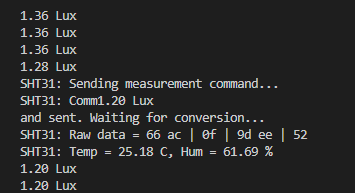
\includegraphics[width=0.7\linewidth]{images/OPT3001_SHT31_OUTPUT.png}
    \caption{UART print statements from OPT3001 and SHT31 sensor}
    \label{fig:sensor_output}
\end{figure}

To validate the current and power readings from the voltage sensors, UART prints were also utilised. Figure~\ref{fig:power_output} shows the ADC values on both ADC channel zero and four, whilst also showing the calculated power. It is to be noted that the power values seen in Figure~\ref{fig:power_output} were from unit testing, are incorrect and are not representative of the final state of the system.

\begin{figure}[H]
    \centering
    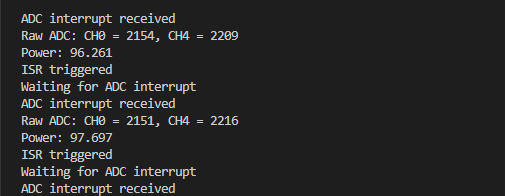
\includegraphics[width=0.7\linewidth]{images/power_uart.png}
    \caption{UART print statements showing raw voltage readings (ADC reading between 0 and 4095) and converted power values (these are initial testing values and the power readings are incorrect)}
    \label{fig:power_output}
\end{figure}

\subsubsection{Testing and Validation: Integrated Tests}
% Describe how real world testing was done for sensors
% photos? Surely figures of UART output or serial plot
% anomalies?

Once the key subsystems were integrated, the raw and filtered outputs of the sensors were plotted using Tauno Serial Plot\parencite{serialplot}. Figure~\ref{fig:integrated-tests} shows that for each different sensor, the EMA filter improves the sensor output versus the raw values with the orange lines representing raw values and the blue lines representing filtered values.

\begin{figure}[H]
    \centering

    \begin{subfigure}{0.45\textwidth}
        \centering
        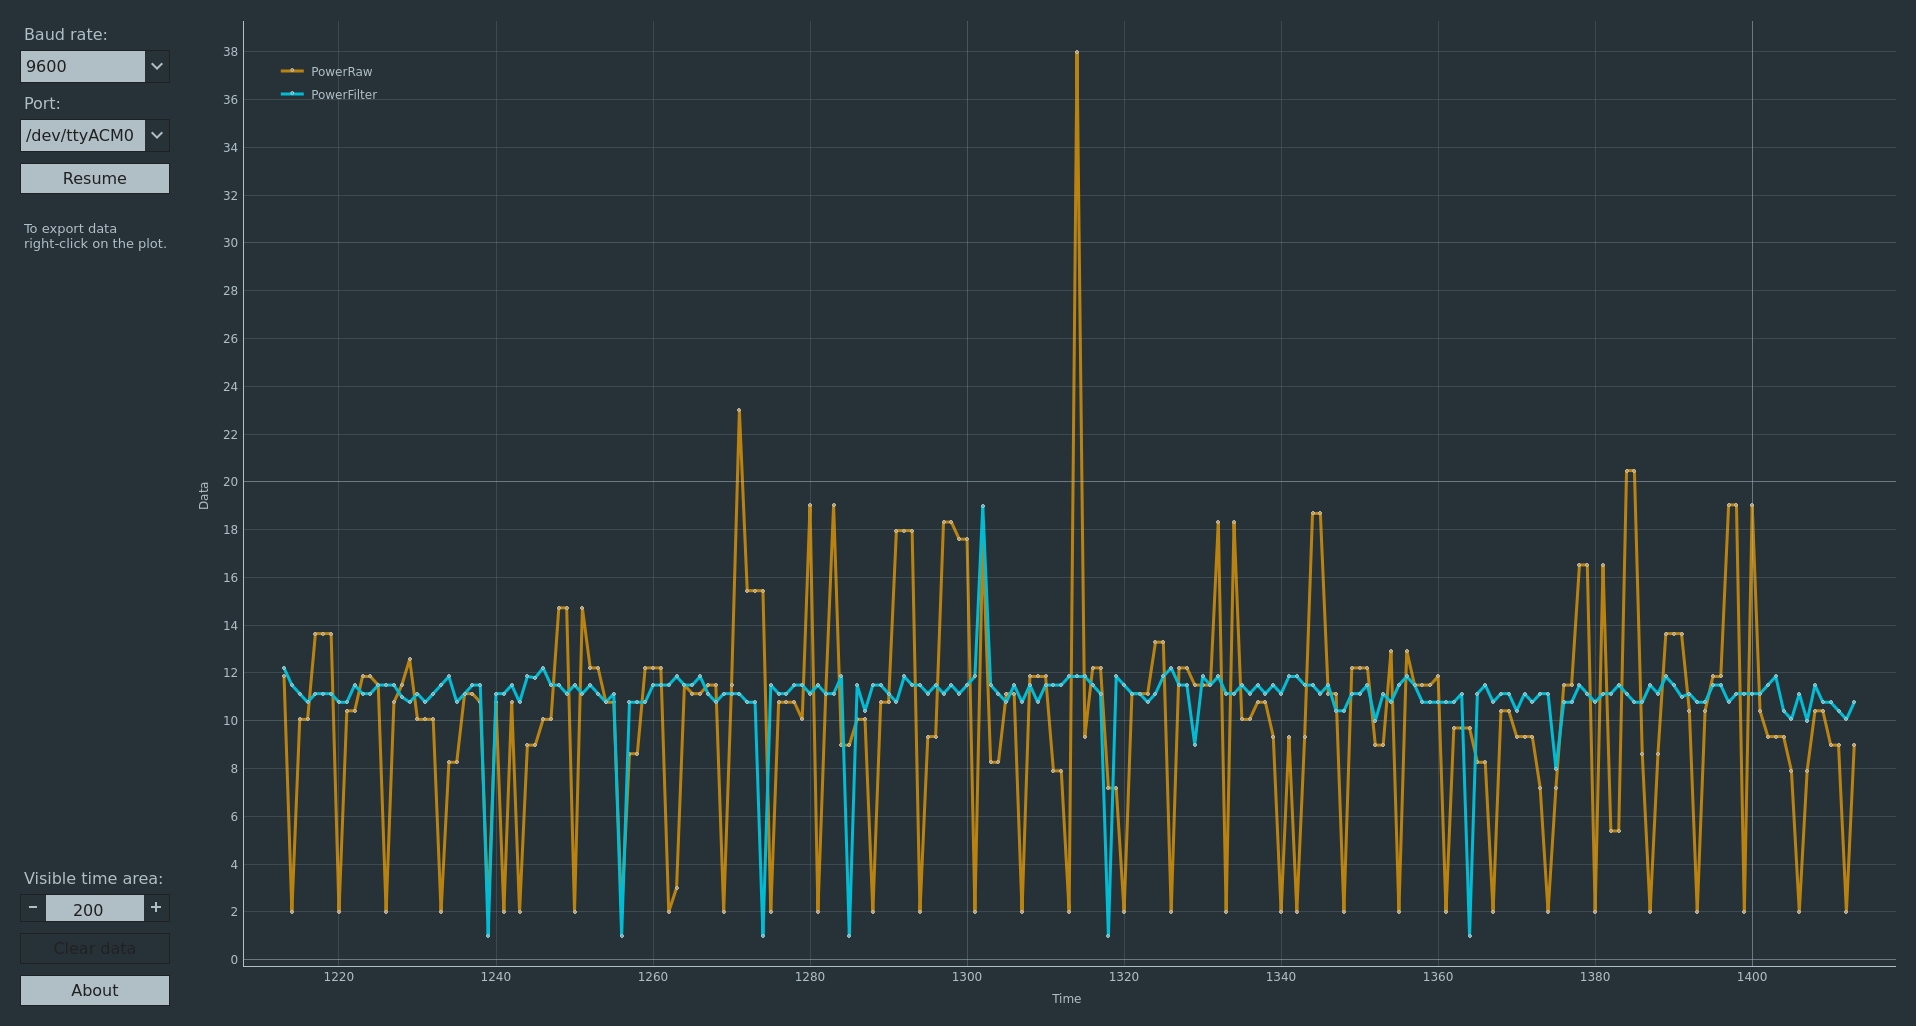
\includegraphics[width=\linewidth]{images/power_serial_plot.png}
        \caption{Raw current values and filtered power values.}
        \label{fig:power_serial}
    \end{subfigure}
    \hfill
    \begin{subfigure}{0.45\textwidth}
        \centering
        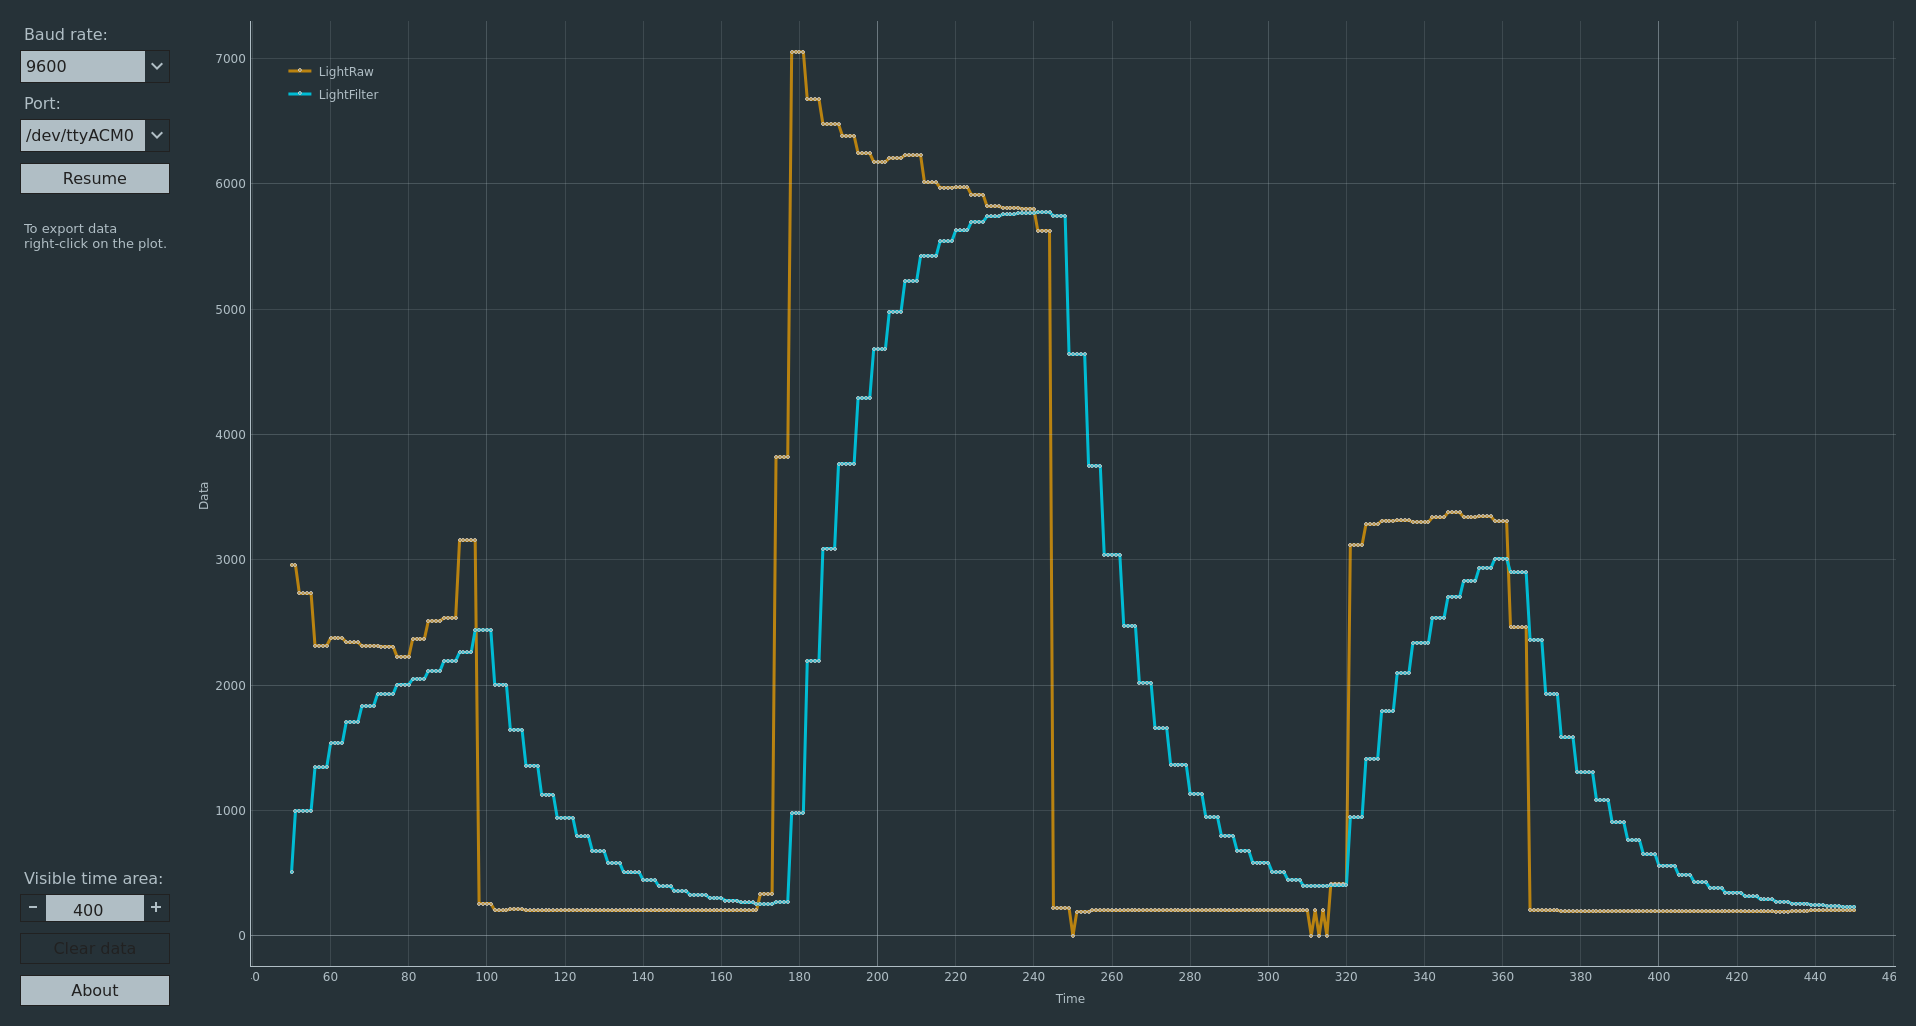
\includegraphics[width=\linewidth]{images/light_serial_plot.png}
        \caption{Raw light values plotted with filtered light values.}
        \label{fig:light_serial}
    \end{subfigure}
    
    \vspace{4mm}

    \begin{subfigure}{0.45\textwidth}
        \centering
        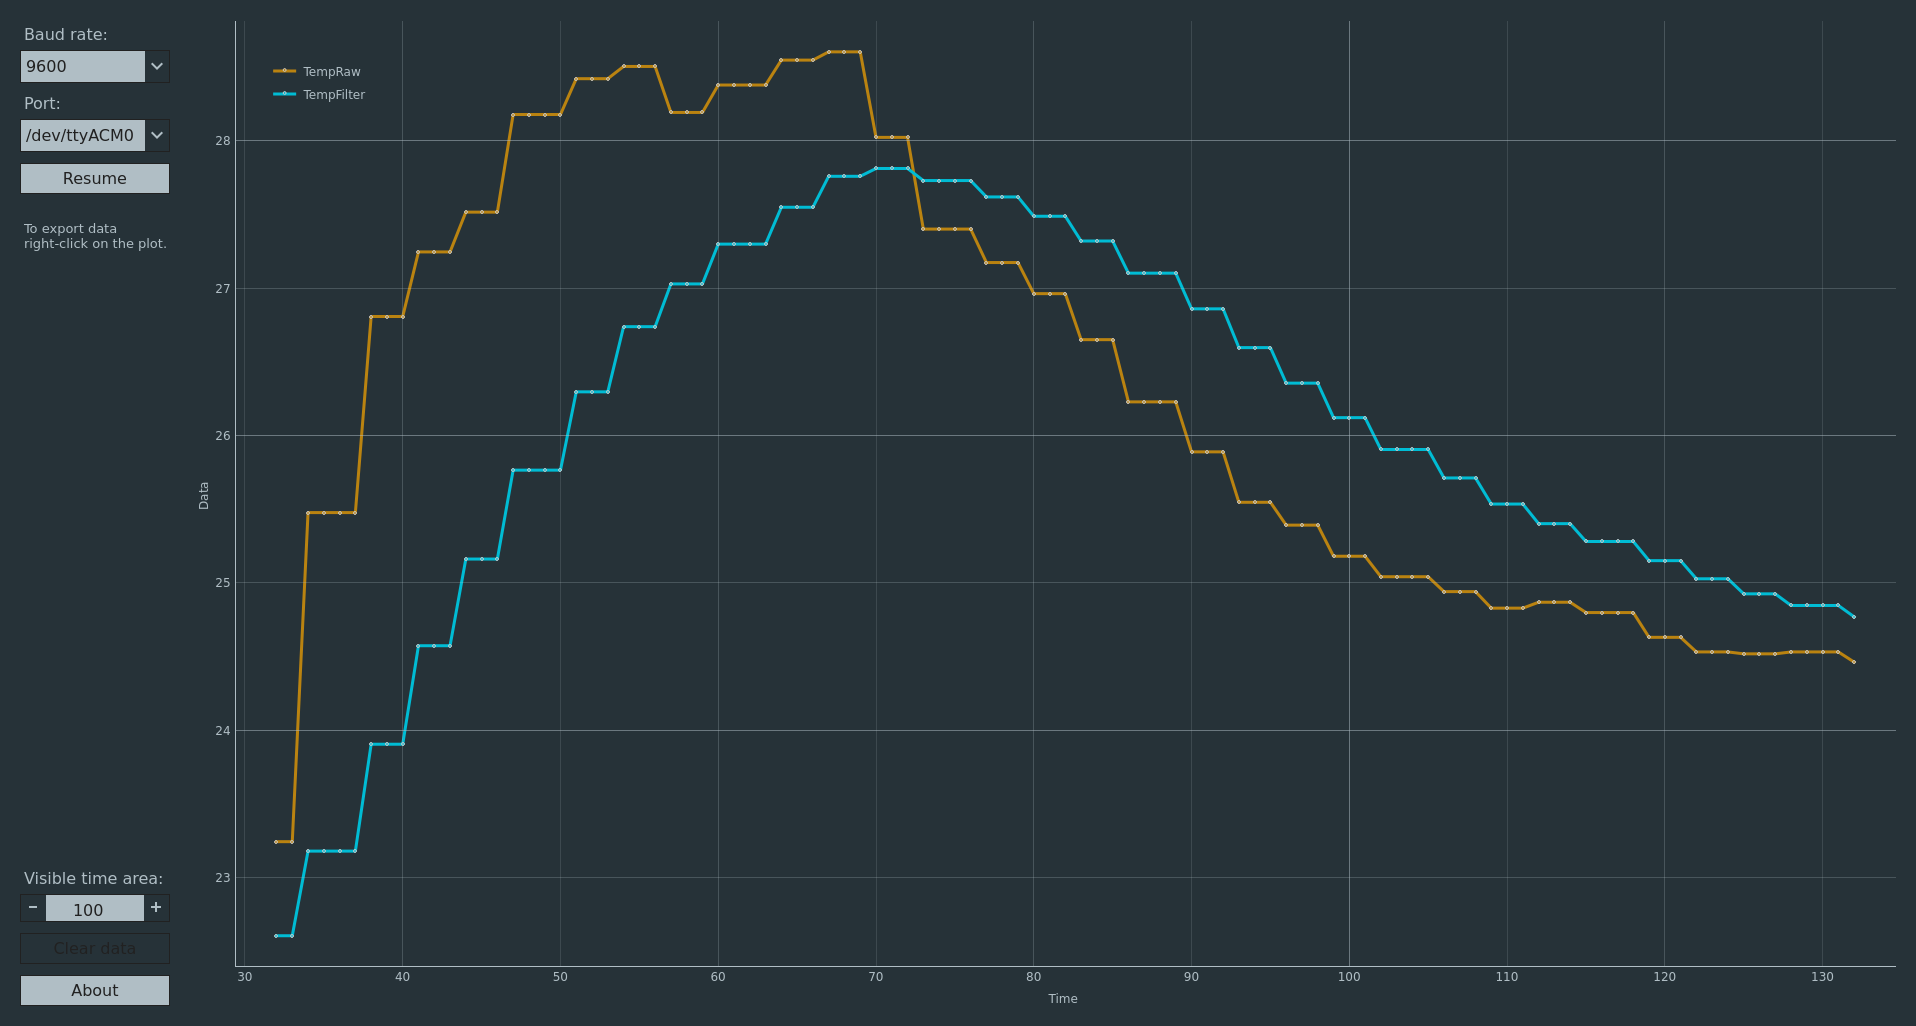
\includegraphics[width=\linewidth]{images/temp_serial_plot.png}
        \caption{Raw temperature values plotted with filtered temperature values.}
        \label{fig:temp_serial}
    \end{subfigure}
    \hfill
    \begin{subfigure}{0.45\textwidth}
        \centering
        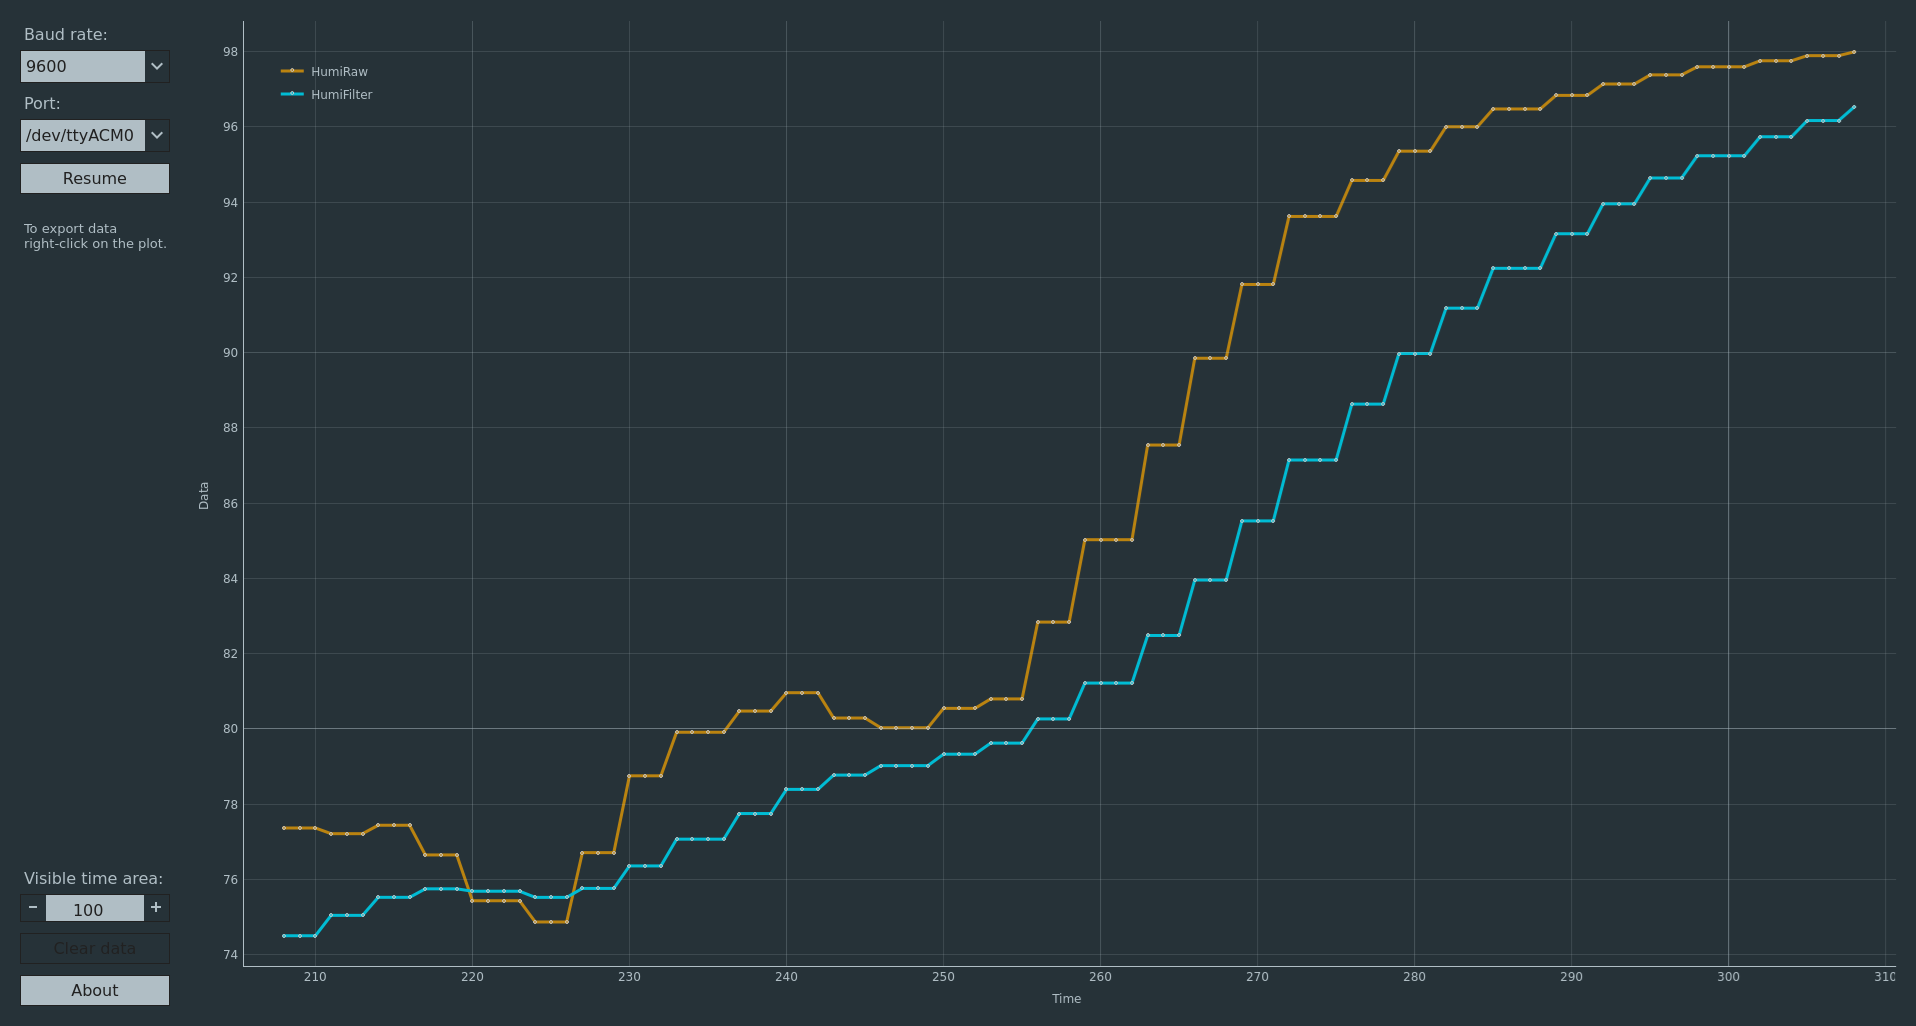
\includegraphics[width=\linewidth]{images/humi_Serial_plot.png}
        \caption{Raw humidity values plotted with filtered humidity values.}
        \label{fig:humi_serial}
    \end{subfigure}

    \caption{Integrated system test runs showing sensor responses under various scenarios.}
    \label{fig:integrated-tests}
\end{figure}


\newpage
\subsection{Graphical User Interface (GUI)}
The graphical user interface (GUI) was designed to provide an intuitive and responsive means of interaction between the user and the embedded system. Its primary functions include monitoring system status, visualising sensor data in real time, adjusting motor parameters, configuring safety thresholds, providing emergency-stop (e-stop) acknowledgement, and displaying sensor plots. Built using the TivaWare Graphics Library (grlib) \parencite{grlib} and widget toolkit, the GUI operates as a dedicated FreeRTOS task and is fully integrated into the task-based system architecture. 

\subsubsection{Design and Task Approach}
The GUI operates on a layered architecture, separating rendering logic from data processing. It runs at ~30 Hz with periodic task delays (vTaskDelay) \parencite{freertos} to balance responsiveness and CPU usage. All rendering is offloaded to a dedicated GUI task, while input data is received asynchronously from other subsystems using FreeRTOS queues and synchronised shared memory (getter() and setter() functions). A separate guiSensorTask filters sensor values and updates canvas widgets for live system feedback.

Touch inputs are handled via the TouchScreenCallbackSet() \parencite{grlib} mechanism and mapped into widget message queues using WidgetPointerMessage \parencite{grlib}, allowing seamless UI interaction without directly polling from the ISR.\\

\subsubsection{Screens, Navigation, and Interface Layout}
The interface comprises of five main screens: Home, Motor, Status, Plots, and Settings. Each are defined in its own canvas widget hierarchy. Navigation is handled through push buttons with callback functions, which dynamically build the desired screen and assigns it to the root widget. The screen management logic is centralised within a dedicated set of functions responsible for constructing and switching between interface screens, enabling modular and scalable navigation throughout the application. Each screen was designed to balance usability with the limitations of the embedded system:
\begin{itemize}
    \item Home Screen: Provides a 2x2 button layout for navigating to each functional screen.
    \begin{figure}[H]
    \centering
    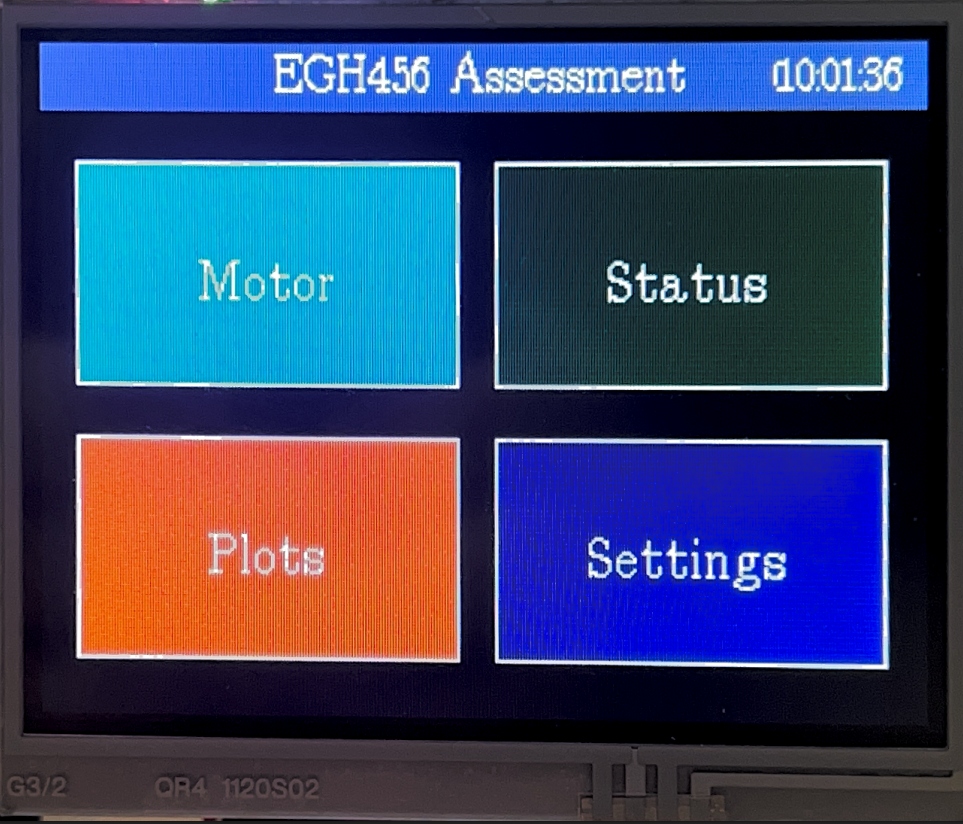
\includegraphics[width=0.7\linewidth]{images/HomeScreen.png}
    \caption{Home Screen Snippet}
    \label{fig:home_screen}
\end{figure}
\item Motor Screen: Includes a toggle button for motor on/off control, a live motor status label, and an RPM slider. The slider updates a global RPM setpoint, used by the control task.
\begin{figure}[H]
    \centering
    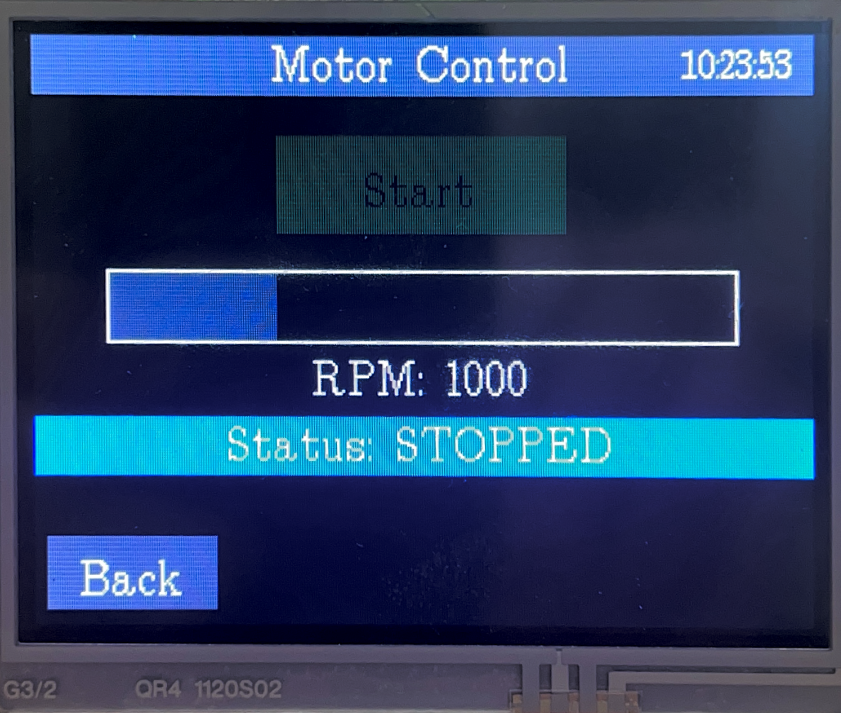
\includegraphics[width=0.7\linewidth]{images/MotorControl.png}
    \caption{Motor Screen}
    \label{fig:motor_screen}
\end{figure}

\item Status Screen\textbf{:} Displays current system metrics (e.g. actual RPM, system mode, power usage), motor state indicators, and safety status.
\begin{figure}[H]
    \centering
    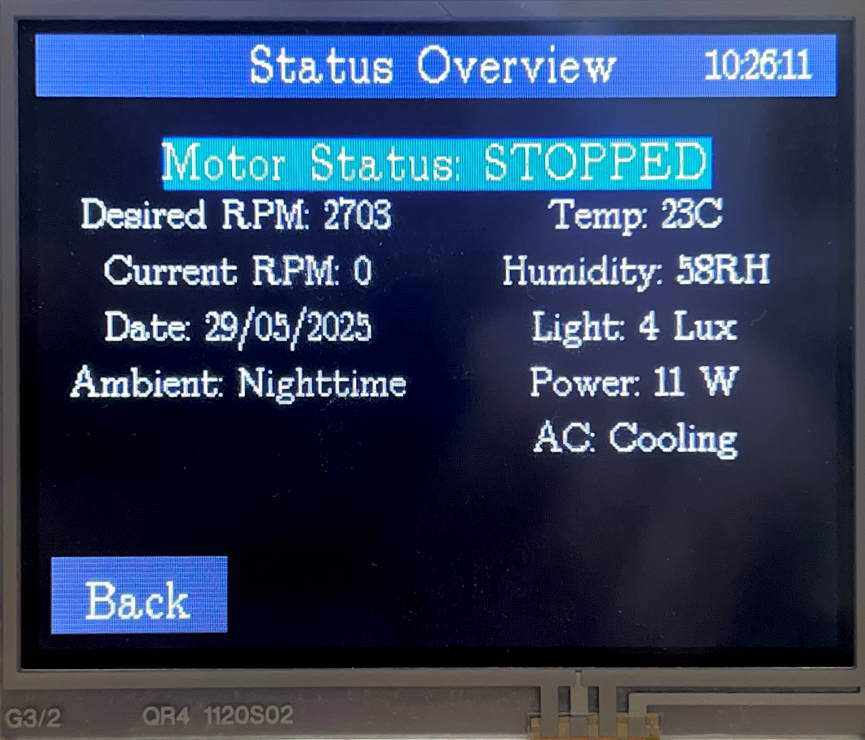
\includegraphics[width=0.7\linewidth]{images/Status.png}
    \caption{Status Screen}
    \label{fig:status_screen}
\end{figure}

\item Plot Screen\textbf{:} Graphs filtered sensor data over time, allowing users to switch between RPM, power, light level, and temperature.
\begin{figure}[H]
    \centering
    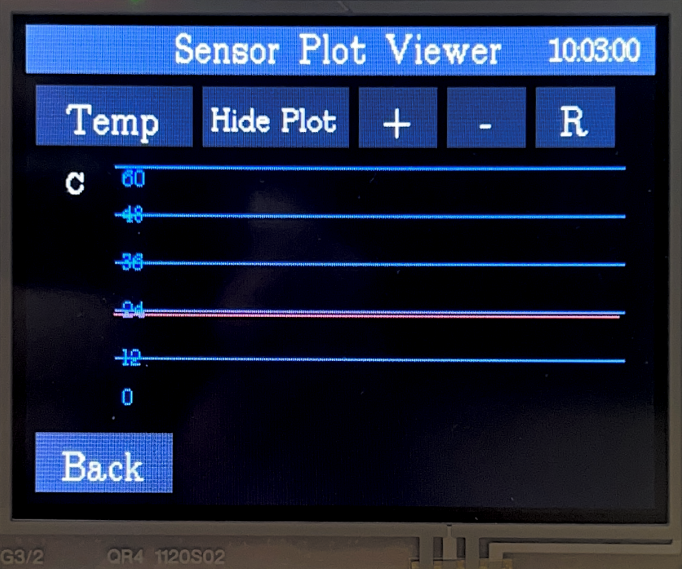
\includegraphics[width=0.7\linewidth]{images/Plot.png}
    \caption{Plot Screen showcasing Temperature}
    \label{fig:plot_screen}
\end{figure}

\item Settings Screen: Allows configuration of upper/lower thresholds for acceleration, temperature, and current via sliders with live numeric feedback.
\begin{figure}[H]
    \centering
    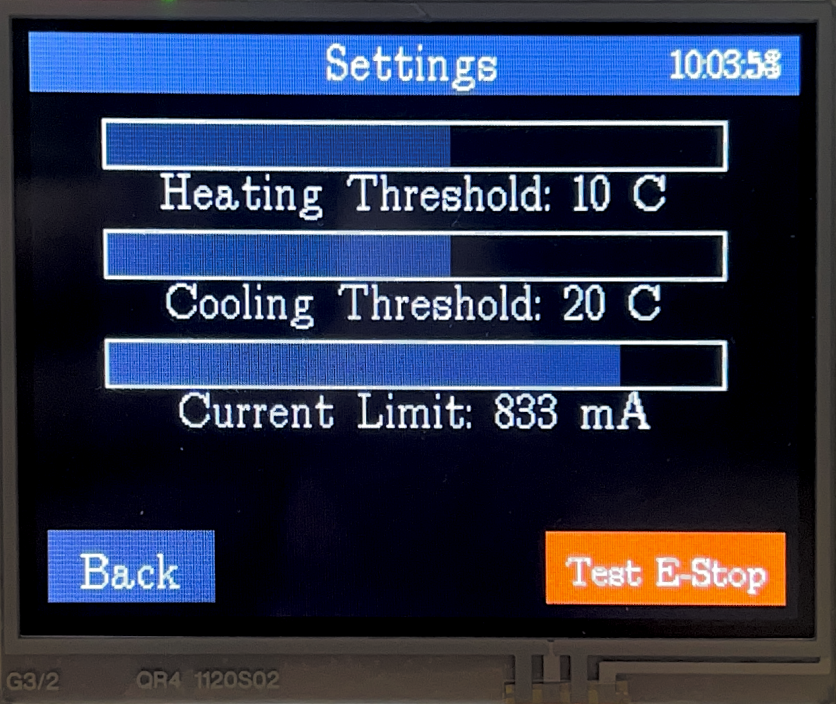
\includegraphics[width=0.7\linewidth]{images/Settings.png}
    \caption{Settings Screen}
    \label{fig:settings_screen}
\end{figure}

\end{itemize} 
Slider inputs update global configuration values via callbacks and are styled for clarity using consistent visual formatting. These inputs directly affect the control and safety subsystems at runtime. \\

\subsubsection{Safety Integration}
When the control system detects a fault (e.g., over current), it sets a global \verb|eStopFlag|. The GUI reacts by disabling motor controls, changing the toggle button to display \textbf{“Acknowledge”} and updating the screen’s visual indicators. The user must manually acknowledge the e-stop via the toggle button; this resets the flag and returns the system to a safe, idle state. This ensures that recovery from fault states is deliberate and traceable.\\
\begin{figure}[H]
    \centering
    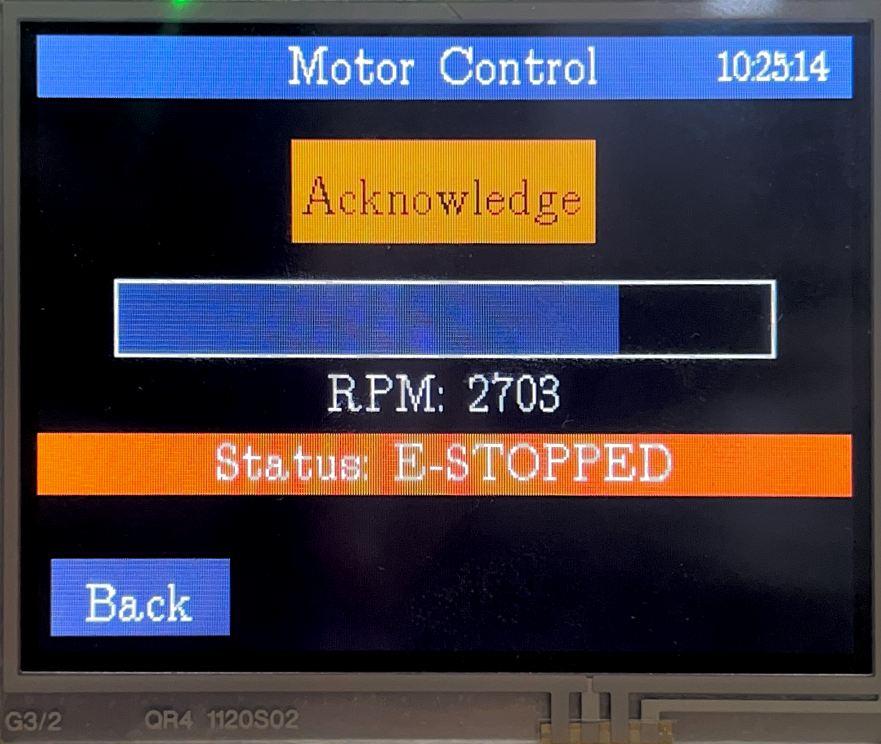
\includegraphics[width=0.7\linewidth]{images/Acknowledge.png}
    \caption{Motor Acknowledge Screen}
    \label{fig:motor_ack_screen}
\end{figure}

\subsubsection{Real-time Clock Implementation}
The GUI displays a real-time clock in the upper-right corner of the Home screen. As the hardware lacks a dedicated real-time clock (RTC), the time is initialised manually to the demonstration day and incremented using a FreeRTOS software timer \parencite{freertos} that triggers once per second. Time is stored in a global structure and rendered using \verb|GrStringDraw()| in the \verb|guiTask|. \\

\subsubsection{Day/Night Detection}
Ambient light is monitored continuously using a light sensor. A value below 5 lux is classified as nighttime. When this condition is detected, the GUI displays a \textbf{“}Night Mode” label and activates a simulated headlight LED on the Status screen. This feature updates every second and could be extended to control physical headlights in a full system implementation. \\

\subsubsection{Sensor-specific Features: Temperature and Humidity}
The selected additional sensor was the temperature and humidity module (SHT31). The GUI displays real-time temperature (°C) and relative humidity (\%RH) values on the \textit{Status} screen, with live updates transmitted via a FreeRTOS queue from the sensor task. Users can configure an upper temperature threshold on the \textit{Settings} screen. If the filtered temperature exceeds this threshold, the AC status message dynamically updates to indicate \texttt{"AC: Cooling"} or \texttt{"AC: Heating"} accordingly. While humidity is continuously monitored and displayed, it does not currently influence system behaviour and is reserved for future feature expansion.\\


\subsubsection{GUI Sensor Plotting}
The Plot screen renders filtered sensor data in real time using a circular buffer. A custom canvas widget calls GUI\_DrawGraph() during PlotPanelPaint() to draw line plots for up to 100 points. Users can cycle through six sensor plots, zoom in/out, reset the Y-axis scale, and toggle visibility. The graphs use labelled axes, consistent colours, and dynamically updated units (e.g., RPM, Lux, °C), supporting fast visual diagnostics.\\

\subsubsection{Hardware and Software Integration}
The GUI subsystem interfaces directly with several hardware components, including a 320x240 pixel LCD display and a capacitive touchscreen panel. The display is driven using a standard graphics controller, while touch input is processed through a dedicated touchscreen module that routes events to the graphical widget system. Analog sensor values, such as current or temperature, are acquired through onboard ADC channels and made available to the GUI for plotting and threshold monitoring. The GUI is built using standard modules from the TivaWare software suite \parencite{grlib}, including the graphics library, widget toolkit, and low-level driver interfaces. Screen layouts are constructed using canvas, slider, and push button widgets, while serial output via the onboard UART is used to support runtime debugging and event logging throughout GUI operation.\\

\subsubsection{Theoretical concepts and Engineering Choices}
The GUI is structured around event-driven programming principles, with a separation between user interface (view), system state (model), and input handling (controller). FreeRTOS tasks follow a producer-consumer model, using queues for communication and avoiding shared memory race conditions through explicit synchronisation. The GUI’s low priority ensures that it remains non-intrusive to motor and sensor threads. Modular design patterns (e.g., one function per screen builder) improve code maintainability and facilitate future expansions such as additional screens or new sensor inputs.


 
\newpage
\section{Results}
\subsection{Motor}
The motor control subsystem demonstrated successful implementation of all key requirements, including real-time phase switching, accurate speed control, safety-compliant acceleration profiles, and reliable emergency stop functionality. Testing was conducted through a combination of hardware validation, UART telemetry logging, and SerialPlot \parencite{serialplot} visualisation to verify system performance under various operating conditions.
\subsubsection{Phase Switching Performance}
Most importantly, the motor demonstrated smooth and quiet operation without whining, stalling, or excessive noise generation. This confirms that the phase switching logic correctly sequences the motor phases in synchronisation with rotor position, preventing the motor from fighting against its own magnetic field. The absence of audible noise or vibration indicates proper timing of phase commutation, which is critical for both motor efficiency and longevity.
\subsubsection{PID Controller Performance}
The PID controller demonstrated effective motor speed regulation under varying load conditions. Through systematic tuning, optimal gains were established that provided:
\begin{itemize}
    \item Rapid response to set-point changes without excessive overshoot
    \item Steady-state accuracy with minimal error between target and actual RPM
    \item Stability under load variations and external disturbances
    \item Smooth operation without oscillation 
\end{itemize}
The conditional PID activation (disabled below 100 RPM) successfully prevented instability during startup and low-speed operation. The kick-start mechanism reliably initiated motor rotation before PID engagement, eliminating startup difficulties that occurred in early testing phases.
Figure \ref{fig:rpm_acceleration} clearly illustrated the PID controller's ability to track the soft RPM reference, with measured RPM following the stepped acceleration profile as designed.
\subsubsection{Safety-Compliant Acceleration}
The acceleration limiting system successfully enforced the 500 RPM/s maximum acceleration requirement and the 1000 RPM/s Emergency stop deceleration. Timer 1A, operating at 50Hz, applied discrete 10/20 RPM increments to achieve the target acceleration/deceleration rate. Testing confirmed:
\begin{itemize}    
    \item Consistent step timing with 20ms intervals between RPM increments
    \item Smooth acceleration curves without abrupt speed changes
    \item Accurate acceleration rates measured at $500\pm10$ and $1000\pm10$ RPM/s
\end{itemize}
The soft RPM approach effectively prevented sudden motor speed changes that could compromise passenger safety or system stability. Visual confirmation through SerialPlot \parencite{serialplot} showed the characteristic staircase pattern of incremental speed changes, validating the controlled acceleration implementation.
\subsection{Sensors}
This results section demonstrates the  performance of the sensor subsystem during system integration and testing. The key outcomes of this section include the verification of sensor accuracy, correct emergency stop activation during over current, and confirmation of stable filtering of sensor outputs. Unit testing and integrated testing was performed to validate this subsystems functionality under real-time conditions. \\

\subsubsection{Sensor Data Validation}
Sensor subsystems were validated when integrating the subsystems. This was done by logging both the raw and filtered sensor values. Each sensor produced expected readings when stimulated. Light levels varied when flashing an external light onto the light sensor, temperature and humidity varied with heat and moisture inputs and current readings increased under high motor loads. By applying EMA filtering \parencite{hunter}, this successfully reduced noise measurements across all sensors.\\

\subsubsection{E-Stop Trigger Validation}
The emergency stop was tested by inducing high current conditions. By loading the motor power supply over its current limit, the e-stop conditions were triggered when the calculated current exceeded the user defined max current limit. Upon e-stop activation, the system began gracefully shutting down the motor via Timer 1A, demonstrating the correct safety response.\\

\subsubsection{Integrated Sensor Plots}

Figure~\ref{fig:integrated-tests} show the representative sensor logs that were captured during the systems operation. Both raw and filtered values are plotted and show current, light, temperature, and humidity readings. These plots show the effectiveness of the EMA filtering approach and demonstrate stable sensor acquisitions for the system.


\newpage
\subsection{Graphical User Interface (GUI)}
The final embedded system successfully fulfilled most functional requirements as specified in the project brief. Core features, including motor control, safety enforcement, sensor monitoring, and real-time GUI interaction, were tested on physical hardware and found to operate reliably under typical conditions.\\

Motor control functionality was verified through the GUI’s start/stop button and RPM slider, which correctly translated user inputs into changes in motor behaviour. Motor speed was reflected in real time via both GUI labels and UART debug output, confirming the integrity of the feedback loop. Safety features were also validated: exceeding the configured temperature threshold reliably triggered an emergency stop, disabling controls and activating a red fault indicator. The system correctly enforced acknowledgement of fault conditions before allowing the motor to restart, as required.\\

The sensor plotting interface performed as expected, displaying smooth and timely graphs of motor speed, estimated power, temperature, and ambient light levels. Users were able to switch between plots, and each graph included labelled axes and colour-coded legends to aid interpretation. Additional features such as the real-time clock and day/night classification were also functional; the software-emulated clock maintained consistency during testing, and light sensor readings correctly toggled the simulated headlight LED under low-light conditions. Threshold adjustments made via sliders were reflected immediately in control logic, demonstrating effective inter-task communication and runtime flexibility.\\

Testing was performed using a combination of interactive GUI checks and UART-based telemetry. Sensor stimuli were simulated manually, for instance, covering the light sensor or applying heat to the temperature sensor, to observe corresponding GUI updates and safety actions. Task behaviour and system state transitions were monitored through log messages and visual feedback, allowing real-time validation of functionality across all modules.\\

Despite these successes, several limitations were identified. Although the humidity sensor was integrated and displayed in the GUI, it was not used in any control logic, reducing its practical contribution. This highlighted the importance of establishing clear functional roles for each sensor during the design phase. Additionally, the plot screen lacked features such as zooming or dynamic scaling, which would have improved data readability in low-variance scenarios. Some code in the GUI module, particularly in \verb|gui.c|, became tightly coupled to global variables, making it more difficult to refactor or extend. A stronger emphasis on modular encapsulation and abstraction could have improved maintainability.\\

These challenges offered valuable lessons in the design of real-time embedded systems, particularly in the balance between responsiveness, usability, and maintainability within resource-constrained environments. Future iterations would benefit from more rigorous interface planning and extended functional roles for all integrated components. Ultimately, the project has demonstrated how embedded systems, when carefully designed and tested, can meet the demanding requirements of electric vehicle applications, therefore providing safe, reliable, and responsive control that is essential for modern transport technologies.

\newpage

\section{Conclusion}
This project successfully delivered a real-time embedded system for controlling an electric vehicle. The system was developed on a Tiva TM4C1294NCPDT microcontroller using FreeRTOS, integrating motor control, sensor acquisition, safety mechanisms, and a graphical user interface into a cohesive and responsive platform.\\

The motor control subsystem met key functional and safety requirements. Though phase switching and feedback-driven speed regulation using a PID controller, the motor responded reliably to changes in user input and load. Acceleration and emergency stop profiles were enforced using timer-based logic, ensuring smooth ramp-up and rapid shutdown without compromising system stability. Phase transitions occurred cleanly, and RPM tracking closely followed the target reference values across a range of operating conditions. \\

Sensor data was acquired through both I2C and ADC interfaces, covering environmental parameters and internal system metrics. Filtering techniques, such as exponential moving averages, significantly improved signal quality, while over-current protection was implemented using real-time power monitoring and an emergency stop trigger. These features were validated through targeted testing and confirmed stable operation in the presence of external disturbances and system noise.\\

The graphical interface supported real-time interaction with the system, offering visual feedback for motor status, sensor values, and safety alerts. Users could adjust control parameters, monitor system performance, and respond to fault conditions through an intuitive touchscreen interface. Additional features such as day/night detection, live plots with zoom controls, and a software-based clock extended system usability while maintaining real-time responsiveness.\\

All system components were developed with a focus on modularity, timing accuracy, and fault tolerance. Subsystems communicated through synchronised shared resources and message queues, with mutual exclusion enforced through mutex protection, thus ensuring consistent behaviour under concurrent execution. Testing confirmed that the system met its design goals, with responsive performance and predictable task scheduling across a range of scenarios.\\

This project demonstrates a practical application of embedded systems engineering principles in a safety-critical context. It highlights the importance of real-time scheduling, reliable sensor integration, and user-focused design in the development of control systems for modern electric vehicles

\newpage
\clearpage
\addcontentsline{toc}{section}{References}
\printbibliography

\onecolumn
\begin{appendices}
\section{Setter and Getter Functions}
\begin{figure}[h!]
\centering
\lstinputlisting[style=cstyle, firstline=26,firstnumber=26, lastline=60]{../src/shared.c}
\end{figure}
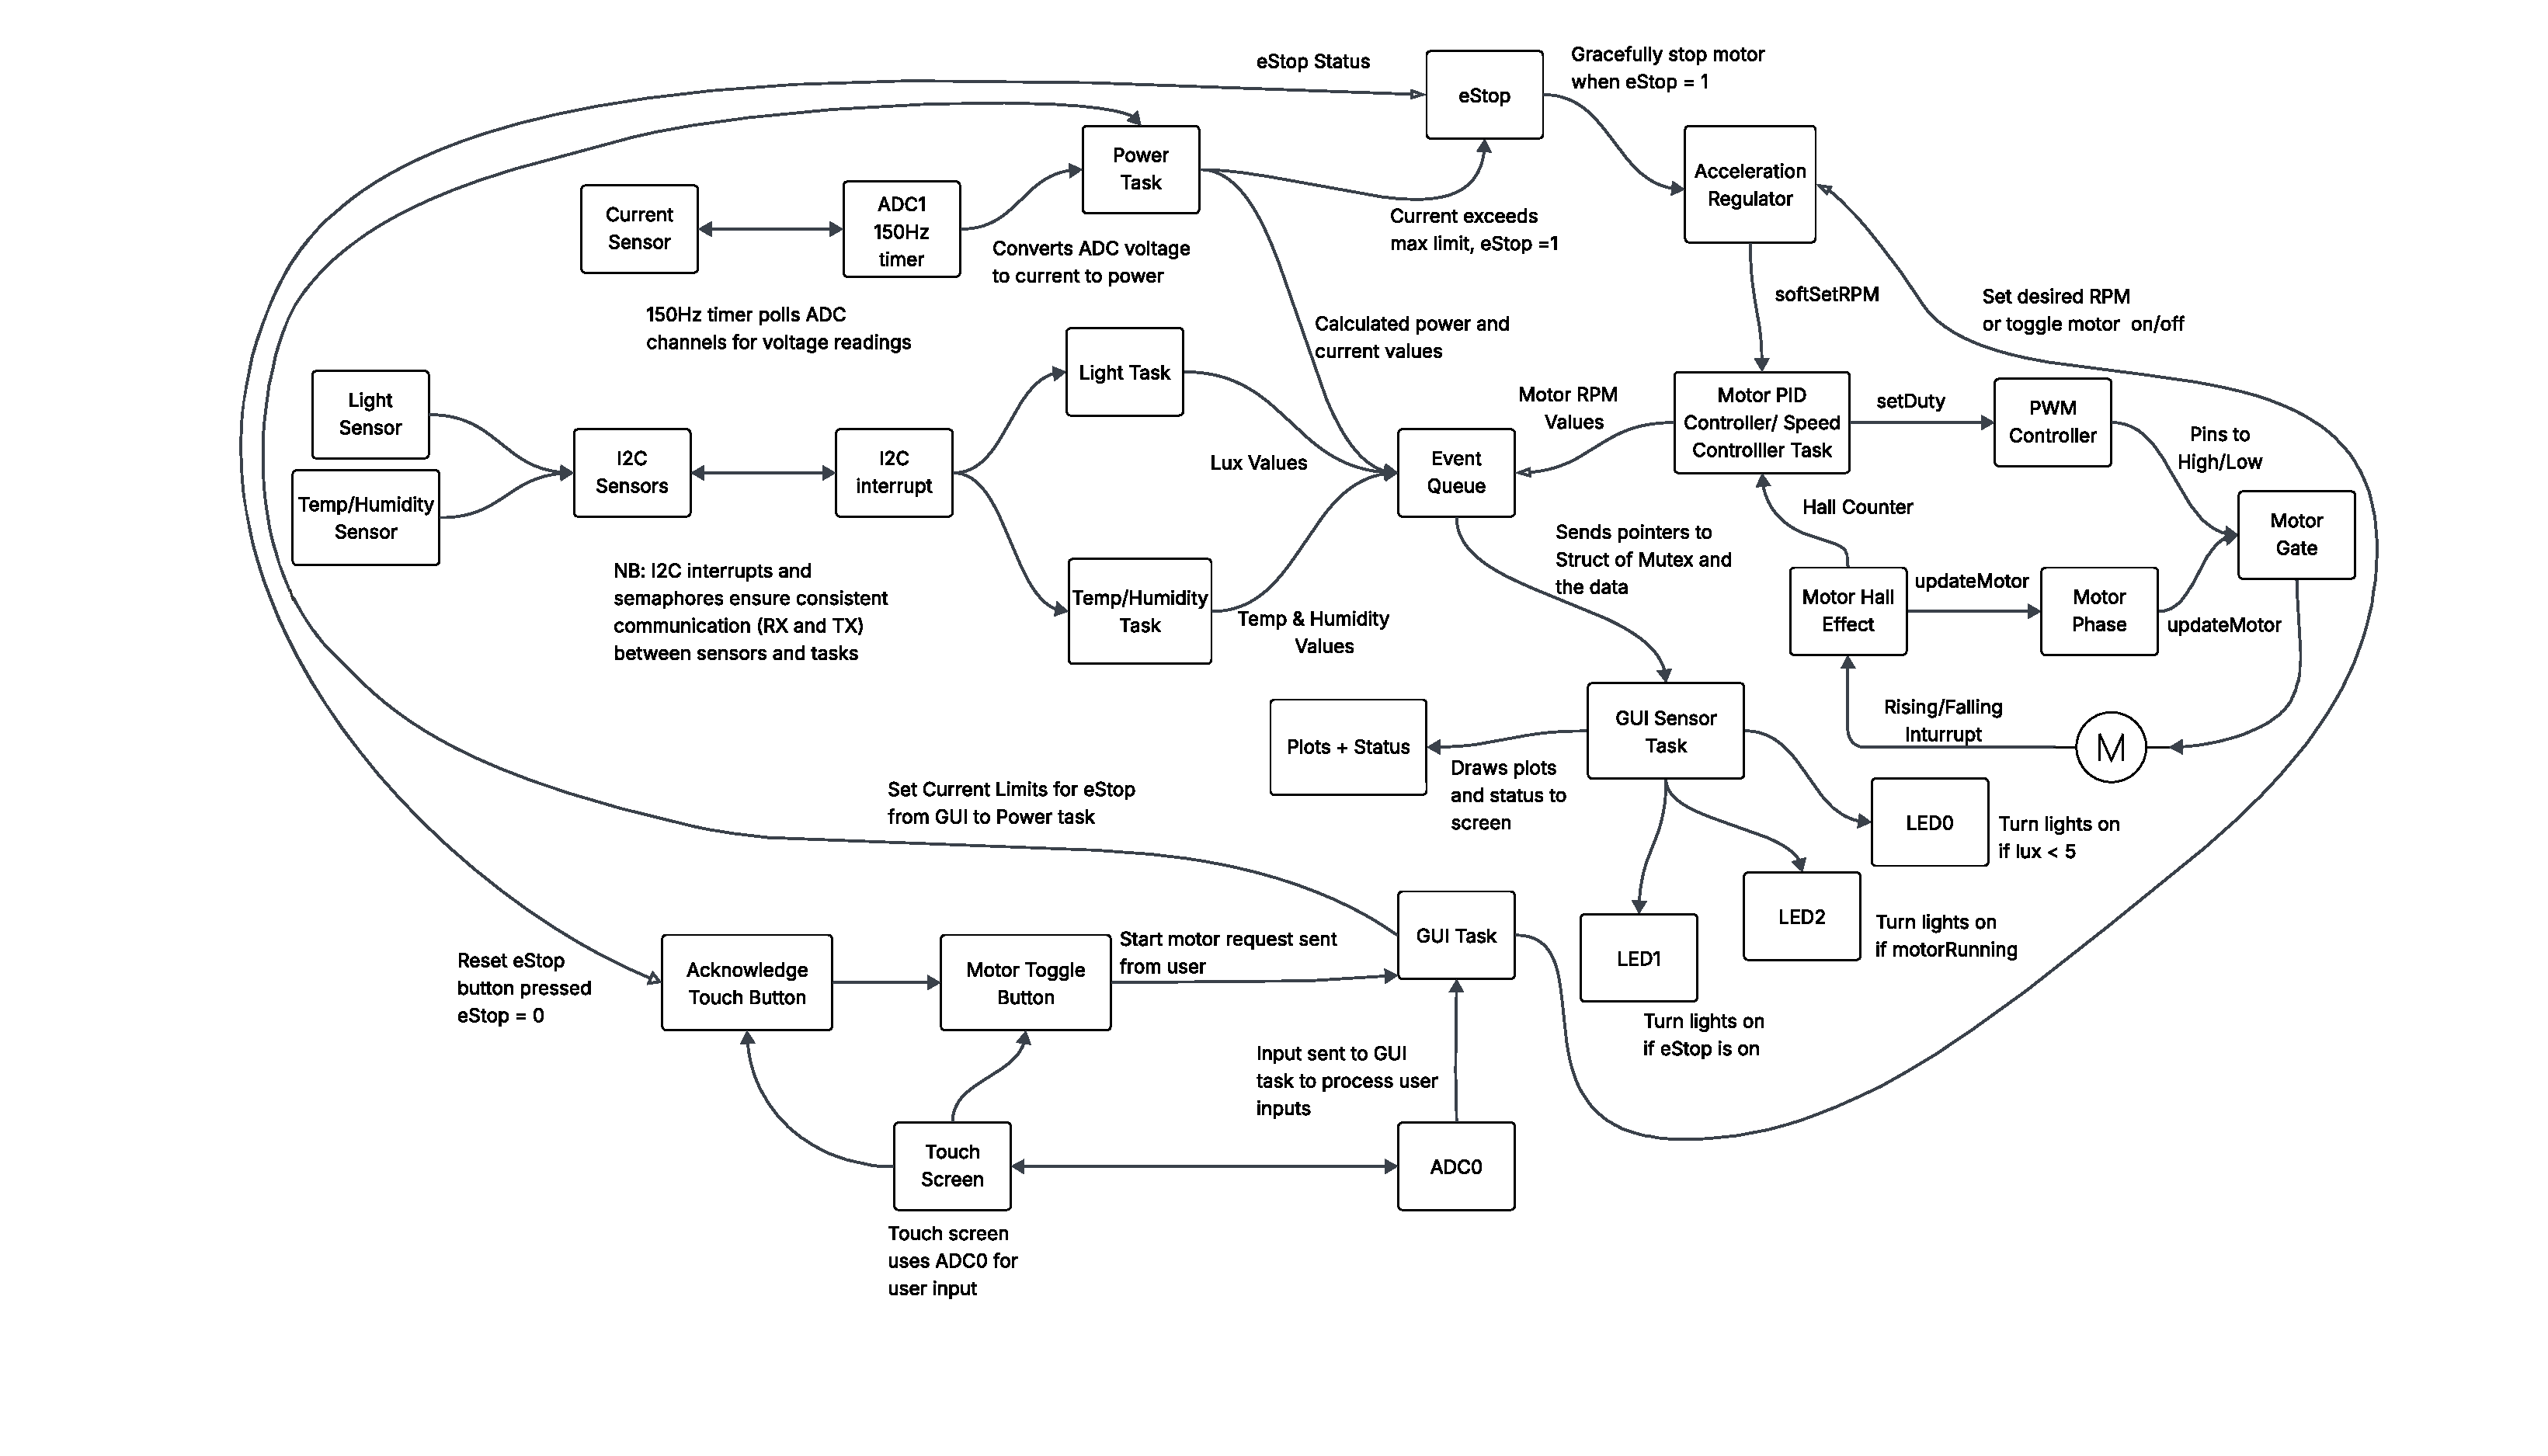
\includepdf[pages=1,angle=270,pagecommand={
    \section{System Architecture}\label{appendix:sysarch}
    \vspace{-2cm}
}]{appendix/sysarch.pdf}
\end{appendices}

\end{document}


